%\documentclass[12pt]{memoireuqam1.3}

% Ajout commentaire pour test par Guy Tremblay

\documentclass[12pt,twoside]{memoireuqam1.3}
% Si vous souhaitez en recto-verso
\usepackage{graphicx}% Pour les figures
\usepackage[french]{babel}
\usepackage[utf8]{inputenc} % Pour utiliser les caractères accentués
\usepackage[T1]{fontenc}
\usepackage{url}
\usepackage{framed}


%----------------------------------------------------------------

%Autres packages et commandes utiles
%----------------------------------------------------------------
\usepackage{amsmath,amsthm,amssymb,amsfonts}	% Pour pouvoir inclure certains symboles et environnements mathématiques
\usepackage{enumerate,enumitem} % Pour mieux gérer la commande enumerate dans les sections
\usepackage{graphicx,multicol}	% Pour inclure des images et les colonnes
\usepackage{array}
\usepackage{color}	% Pour inclure du texte en couleur
\usepackage{units}	% Pour pouvoir tapper les unités correctement
\usepackage{pgf,tikz}	% Utilisation du module tikz, qui permet de tracer des belles images
\usetikzlibrary{arrows} % Quand on exporte une image GeoGebra, on a besoin de préciser cela
\usepackage{hyperref}	% Pour include des liens dans le document
\newcommand{\N}{\mathbb{N}}	% Commande personnelle, plus rapide pour taper les ensembles
\newcommand{\Z}{\mathbb{Z}}	% Commande personnelle, plus rapide pour taper les ensembles
\newcommand{\R}{\mathbb{R}}	% Commande personnelle, plus rapide pour taper les ensembles
\usepackage{cprotect}	% Pour pouvoir personaliser la légende des figures
\usepackage{float} % Pour pouvoir utiliser d'autres placements de figures tels que H (HERE forcé h!)
\usepackage{subcaption}
\usepackage{comment}
\usepackage[square,numbers]{natbib}

%%%%%%%%%%%%%%%%%%%%%%%%%%%%%%%%%%%
% Items, and Enum

\newcommand{\GT}[1]{{{\textcolor{red}{\footnotesize [[(Guy T.) #1]]}}}}
\newcommand{\gt}[1]{}

\newcommand{\EH}[1]{{{\textcolor{green}{\footnotesize [[(Ellen) #1]]}}}}
\newcommand{\eh}[1]{}

\newcommand{\ACOMPLETER}[1]{{{\textcolor{blue}{\small #1}}}}

\newcommand{\AVERIFIER}[1]{{{\textcolor{orange}{\small (A v\'erifier!!) #1}}}}


%%%%%%%%%%%%%%%%%%%%%%%%%%%%%%%%%%%



%Création du glossary (liste des acronymes)
\usepackage[toc,section=chapter,acronym,nomain]{glossaries}
\makeglossaries

% Marquage des chapitres dans la liste des figures
\usepackage{etoolbox}
\preto\figure{%
  \ifnum\value{figure}=0\addtocontents{lof}{{\bfseries Chapter \thechapter\vskip10pt}}\fi
}


\begin{document}
%%%%%%%%%%%%%%%%%%%%
% Pour la page titre
%%%%%%%%%%%%%%%%%%%%
\title{Game Genesis \hspace{20cm} Un profil UML pour la conception de jeux vidéos}
% Votre nom complet tel qu'il apparaît à votre dossier du registrariat de l'UQAM
\author{Ellen Haas}
% Année et mois courant sauf si spécifié autrement pas \degreemonth et \degreeyear
%\degreemonth{mois du dépôt}
%\degreeyear{année du dépôt}
\uqammemoire %% ou \uqamthese ou \uqamrapport
\matiere{informatique}
\thispagestyle{empty}        % La page titre n'est pas numérotée
\maketitle



%%%%%%%%%%%%%%%%%%%%
% Page préliminaires
%%%%%%%%%%%%%%%%%%%%
\renewcommand \bibname{R\'EF\'ERENCES}% FACULTATIF
%si vous voulez qu'apparaisse le titre RÉFÉRENCES plutôt que BIBLIOGRAPHIE
\renewcommand \listfigurename{LISTE DES FIGURES}
\renewcommand \appendixname{APPENDICE}
\renewcommand \figurename{Figure}
\renewcommand \tablename{Tableau}

\pagenumbering{roman}  %% numérotation des pages liminaires en chiffres romains
\addtocounter{page}{1} %% les remerciements commencent à la page ii
%\chapter*{Remerciements}


Tout d'abord je souhaite remercier mon directeur de recherche, Guy Tremblay.
Pour sa présence, son temps ainsi que sa patience tout au long de ma maîtrise.
Je souhaite aussi le remercier pour la confiance qu'il m'a accordée lorsque je lui ai proposé un sujet de recherche de ma propre initiative.
Ses conseils et son expérience m'ont accompagnée tout au long de ma recherche et de ma rédaction.


Je souhaite également remercier mon conjoint, Jehan.
Il m'a encouragée dans les moments de travail intense, épaulée durant les moments compliqués et m'a secouée dans les moments où je ne pensais plus y arriver. 
Ses paroles rassurantes, ses encouragements bruyants et la confiance inébranlable qu'il a exprimée tout au long de cette maîtrise ont été pour moi le socle solide qui m'a permis de continuer.


Je souhaite également remercier des professeurs qui ont joué un rôle important dans ma vie.
M.~Flieg qui a su rallumer en moi l'envie d'étudier et de découvrir de nouvelles choses en appréhendant le monde sous un angle différent.
M.~Froeliger sans qui j'aurais abandonné l'idée de faire mon échange à l'UQAM avant même d'être venue.


Je remercie également mes amis.
Qu'ils soient tout près ou très loin.
Que je les côtoie toutes les semaines ou que je les voie rarement.
Ils sont nombreux, je ne les citerai donc pas, mais ils se reconnaîtront.


Enfin je tiens à remercier ma famille.
Mon père tout d'abord, sans qui rien n'aurait été possible.
Pour la confiance qu'il m'accorde, pour la patience dont il a toujours fait preuve et pour son soutien au quotidien depuis de nombreuses années.
Je remercie également ma grande soeur qui, même si elle est loin, a toujours un oeil sur ce que je fais.

%\chapter*{Dédicace}
\begin{flushright}
\begin{small}

Je dédie ce mémoire à mon fils, Nahel. 
\\Pour que tu puisses avoir la même chance que moi
\\de faire tes propres choix dans la vie.
\\Pour que je puisse te soutenir et t'épauler 
\\dans le chemin que tu suivras 
\\comme ton grand père l'a fait pour moi.

\end{small}
\end{flushright}

%\chapter*{Avant-propos}

\tableofcontents % Pour générer la table des matières
\listoffigures % Pour générer la liste des figures
\listoftables % Pour générer la liste des tableaux
\newacronym{gg}{GG}{\emph{Game Genesis}}
\newacronym{dlc}{DLC}{\emph{Downloadable Content}}
\newacronym{gdd}{GDD}{\emph{Game Design Document}}
\newacronym{esrb}{ESRB}{\emph{Entertainment Software Rating Board}}
\newacronym{usp}{USP}{\emph{Unique Selling Points}}
\newacronym{ia}{IA}{\emph{Intelligence Artificielle}}
\newacronym{mda}{MDA}{\emph{Mechanics Dynamics Aesthetics}}
\newacronym{dpe}{DPE}{\emph{Design Play Experience}}
\newacronym{dde}{DDE}{\emph{Design Dynamics Experience}}
\newacronym{fps}{FPS}{\emph{First Person Shooter}}
\newacronym{uml}{UML}{\emph{Unified Modeling Language}}



\printglossary[title=LISTE DES ABRÉVIATIONS\, DES SIGLES ET DES ACRONYMES]

\begin{abstract}

\gt{Dans le cadre du mémoire, tu décris <<ce que tu as fait>>. Il est donc
généralement préférable d'utiliser le passé plutôt que le futur.}

\gt{Oops! Comme indiqu\'e hier, j'ai des probl\`emes avec mon MacOS --
au niveau du termial utilis\'e.  J'utilise donc un nouveau
terminal. Le bon point: il me permet de voir correctement les accents,
et donc spontan\'ement j'en ai mis quelques-uns... jusqu'\`a ce que je
r\'ealise que peut-\^etre que toi, sur Windows, tu ne les vois pas
correctement.  Donc, je continue \`a utiliser des accents \LaTeX, mais
si tu vois des caract\`eres bizarres dans le dernier commit ou dans le
r\'esum\'e, c'est a cause de cela.}

\eh{Je travaille sur overleaf, donc les accents \'e et é sont tous deux pris en charge sans soucis}


\gt{Ci-bas: j'ai simplifi\'e un peu, car le r\'esum\'e me semblait un peu long.}

Le développement de jeux vidéos est un domaine en pleine expansion.
Les jeux deviennent plus complexes,
les projets plus compliqués, les budgets plus importants, les d\'elais de développement plus serr\'es.
Afin d'accélérer les étapes du développement d'un jeu, de nombreux outils émergent~: 
 moteurs de jeu, environnements de développement intégrés, outils de gestion de projet, logiciels de création 3D, aide au développement d'intelligences artificielles, gestion des animations, etc.
Cependant, un pan complet de la création de jeux vidéos reste encore peu formalisé et peu outillé : le~\emph{game design}.
%
Pourtant, la réflexion sur le~\emph{game design} et la documentation des concepts d'un jeu vidéo sont des étapes cruciales.
Sans une solide documentation et des concepts clairement énoncés, un projet de développement peut être rapidement voué à l'échec.

Dans le cadre de notre recherche,
nous avons cherché à identifier les bonnes pratiques de rédaction d'un~\emph{Game Design Document} ainsi que les outils utilisés pour les étapes de~\emph{game design} et de pré-conception.
Comme r\'esultat de ce travail, nous proposons~\emph{Game Genesis}, un profil UML pour faciliter la rédaction d'un~\emph{Game Design Document}.

UML introduit un langage formel, une structure précise, des outils performants et un support de communication efficace.
Le domaine du développement de jeux vidéos est cependant très vaste. 
La taille des équipes de développement, les genres de jeux vidéos, les types de~\emph{gameplay}, les spécificités de~\emph{game design} entraînent une difficulté à anticiper tous les éléments nécessaires à la rédaction d'un \emph{Game Design Document}.
La liste des \'el\'ements introduits dans~\emph{Game Genesis} est donc non exhaustive et ces éléments sont assez généraux afin de ne pas faire obstacle à la représentation de certains types de jeux vidéos.

\gt{Ci-haut: un peu trop tot (contexte insuffisant) pour parler de
<<st\'er\'eotypes>>, donc <<\'el\'ements>> devrait suffire.}

Afin de structurer le profil \emph{Game Genesis}, nous avons fait usage du~\emph{Framework MDA}, qui sépare le~\emph{game design} en trois aspect~: \emph{Mechanics}, \emph{Dynamics} et \emph{Aesthetics}.
Plus sp\'ecifiquement, avec~\emph{Game Genesis}, nous proposons un profil pour aider \`a mod\'eliser les \'el\'ements de~\emph{Mechanics} d'un jeu vidéo.
%
Nous illustrons l'utilisation de ce profil en mod\'elisant les
\'el\'ements de \emph{Mechanics} de PUBG (\emph{PlayerUnknown's
Battlegrounds}), un jeu vid\'eo populaire sorti en 2017.


MOTS CLÉS :~\emph{Game design}, jeux vidéos,~\emph{Game Design Document},~\emph{Framework MDA}, profil UML.

\end{abstract}







% Utilisez l'environnement  abstract pour rédiger votre résumé


%%%%%%%%%%%%%%%%%%%%
% Document principal
%%%%%%%%%%%%%%%%%%%%

\begin{introduction}


De nombreux défis entourent le développement de jeux vidéos et les outils et méthodes pour y parvenir sont variées.
Cependant, il devient de plus en plus important de chercher des méthodes afin d'accélérer le développement, sans pour autant impacter la qualité du contenu final.
Un \emph{Game designer} se doit d'être précis et concis dans ses descriptions et ses communications afin de transmettre un maximum d'informations et de pouvoir dédier plus de temps à l'exploration, à la recherche artistique et au développement d'un prototype. 

%quoi
Dans ce mémoire, nous allons présenter \gls{gg} (cf.~Section~\ref{game-genesis.sect}), un profil UML (cf.~Section~\ref{profils-UML.sect}) qui permet d'outiller le processus de pré-conception d'un jeu vidéo, facilitant ainsi la documentation et la rédaction des documents descriptifs du jeu vidéo en cours d'élaboration.

%rapidité
Destiné à être utilisé dans les premières phases du développement, \emph{Breaktrough} et Pré-conception~\ref{prob.etapes}, ce profil UML permet l'accélération de la documentation à travers un outil visuel représentant les mécaniques et les objets du jeu.
Ceci permet de produire un prototype jouable plus rapidement.

%cohérence
L'utilisation d'un profil UML permet d'apporter une structure précise et un cadre de travail rigoureux lors de la conception afin d'assurer la cohérence des modèles durant toute leur durée de vie.

%maintenance & modifications
Lors de sa conception, un jeu vidéo est destiné à évoluer rapidement et sa documentation se verra modifiée de nombreuses fois afin de toujours être la plus pertinente possible.
Le standard UML --- \gls{uml} --- permet d'apporter un support visuel à cette documentation et permet également de rendre les modifications plus faciles en accédant aux objets concernés rapidement et efficacement. 

%pérennité
Effectuer des \emph{mind mapping} est un moyen simple et efficace permettant d'illustrer des idées de manière visuelle.
Cependant, le manque de rigueur (modifications erratiques, contenu incohérents, manque de structure) et les supports utilisés (feuille de papier ou tableau) lors d'un travail de \emph{mind mapping} n'assurent pas du tout la pérennité des informations stockées.
Bien qu'il existe des logiciels de \emph{mind-mapping} qui conservent les informations sous la forme d'un fichier XML, il n'existe pas réellement de <<~standard~>> définissant de manière formelle un langage de \emph{mind-mapping}.
De plus, chaque outil de \emph{mind-mapping} possède ses propres notations, méthodes et représentations.

De par sa structure imposée et précise, le standard UML permet de structurer les données, de les stocker sous un format précis et de les maintenir facilement en communiquant sur les modifications effectuées.
Ceci permet un stockage beaucoup plus pérenne des informations contenues dans le modèle.

\gt{Il faudra r\'eviser ce qui pr\'ec\`ede: on peut aussi utiliser un
outil logiciel pour cr\'eation de Mind Maps, par ex., FreeMind, qui
conserve le MindMap sous forme XML.  N'en reste pas moins un
d\'esavantage: ce n'est pas un standard, i.e., chaque outil de
MindMapping a son propre format, ses propres variantes et
repr\'esentations, etc. J'ai l'impression que c'est plus de ce cot\'e
qu'il faut argumenter, que sur l'aspect papier/photos des mind maps.}


%réutilisation
UML étant un langage de modélisation largement utilisé et approuvé dans le domaine informatique, il est possible d'utiliser de nombreux outils existants, d'assurer son intégration et sa réutilisation dans différents cadres et sous différentes formes.

%gdd
Un modèle UML pourra également servir de support à la rédaction d'un \gls{gdd}~\ref{sect.GDD}, en organisant les mécaniques de jeu sous forme de catégories réutilisables.
Le GDD est la <<~bible du design~>>~\cite{GD_foundations_pedersen} du jeu.
Il permet de définir tout le contenu du jeu et toutes les informations nécessaires à son développement, et ce sur toute sa durée de vie. 

%generation de code
UML étant reconnu comme langage de modélisation de logiciels, il peut également être possible d'utiliser les modèles créés en pré-conception afin de faciliter le développement informatique du jeu.
Le modèle peut permettre de créer une structure de projet ou du pseudo code pouvant servir de squelette en début de développement.
\end{introduction}


% Utilisez l'environnement  introduction pour rédiger votre introduction
\chapter{Le développement de jeux vidéos}

\label{chap.dev_jv}
Dans le pr\'esent chapitre, nous pr\'esentons les concepts cl\'es
li\'es au d\'eveloppement de jeux vid\'eos, notamment, les \'etapes de
cr\'eation d'un jeu, la distinction entre exploitation et exploration,
les moteurs de jeux, les types de \emph{gameplay}.
%
Mais, dans un premier temps, nous pr\'esentons une notion qui revient
souvent dans les sections qui suivent, celle de \emph{gameplay}.



\section{La notion de \emph{gameplay}}

Le \emph{Gameplay} d'un jeu vidéo est la façon dont le joueur se servira des éléments du jeu pour avancer vers le but du jeu.
Le joueur définit une stratégie et met en place les éléments comme il le souhaite afin de remplir les objectifs du jeu auquel il joue.
Dans un MMORPG (Genre de jeux vidéo définit dans la Section~\ref{MMORPG}) une mécanique de \emph{gameplay} serait :
\begin{itemize}
    \item Je suis un guerrier
    \item Je suis contre un boss effectuant des attaques de glace
    \item Ce boss est sensible aux attaques de feu
    \item En toute logique j'équipe mon personnage en conséquence
    \item J'équipe une armure A me défendant contre la glace et une arme A faisant des dégâts de feu
\end{itemize}
Cependant Rolling et Morris~\cite{Rollings2004} avancent qu'une mécanique de \emph{gameplay} doit éviter d'être triviale afin de pouvoir laisser le choix à un joueur d'adapter sa stratégie en fonction de nombreuses caractéristiques.
Cela peut amener à des choix qui semblent moins évident mais qui deviennent plus efficaces sur le moment en fonction des éléments réunis dans le combat.
Prenon le cas précédent de notre boss de glace.
\begin{itemize}
    \item Le joueur sait que le boss a une seule attaque de glace dévastatrice
    \item Sur un équipement (Armure B) il a la possibilité d'annuler cette capacité du boss
    \item Cette Armure B possèdes des statistiques de protection contre la foudre et d'augmentation de dégâts
\end{itemize}
Le joueur se retrouve alors devant deux choix qui peuvent sembler corrects :
\begin{itemize}
    \item Équiper l'Armure A afin de se protéger et limiter les dégâts du boss
    \item Équiper l'Armure B, annuler l'attaque de glace du boss, tuer le boss plus rapidement avec l'augmentation de ses dégâts. 
\end{itemize}
Les deux cas sont à prendre en compte par le joueur car ils ont chacun leurs avantages et leurs inconvénients.
C'est ce type de choix, selon Rolling et Morris~\cite{Rollings2004}, qui apportent un \emph{gameplay} riche et intéressant dans un jeu vidéo.
Ils avancent même à un moment que l'équilibre entre plusieurs \emph{gameplay} est réellement important dans un jeu vidéo.

Une option présente dans le jeu mais n'a aucun intérêt d'être jouée est une erreur de \emph{game design} et ils la qualifient de <<~Stratégie dominée~>>.
Dans la même optique une option présente dans le jeu qui semble être la seule viable, la plus puissante de toute ou une option supérieure à toutes les autres peu importe les facteurs extérieurs est qualifiée de <<~Stratégie dominante~>>,

Un type de \emph{gameplay} réellement plus puissant que les autres enlèverai une partie du <<~Fun~>> ressentit par le joueur, car ce ne serait plus une question de choix, mais juste une question de calculs.
Les personnes souhaitant faire le choix d'une stratégie moins évidente et moins \emph{mainstream} serait désavantagées par une mécanique de \emph{gameplay} trop forte par rapport aux autres.
C'est ce que Rolling et Morris~\cite{Rollings2004} qualifient de <<~Problème de la stratégie dominante~>>. 
Afin de contrer ce problème ils avancent que laisser la marge de manoeuvre plus grande aux joueurs permet d'éviter ce soucis en leur permettant de construire leurs propres stratégies.
Ils considèrent que <<~Un jeu bien designé ne devrait pas contenir d'options qui ne valent pas la peine d'être jouées~>>.

Mais ils précisent qu'une option de \emph{gameplay} n'est pas un simple choix logique.
Une mécanique de \emph{gameplay} doit être réfléchie et composée de nombreuse règles afin de pouvoir permettre la présence de plusieurs stratégies viables dans un même cas donné.

Chaque choix doit avoir ses avantages et ses inconvénients propres afin que le joueur puisse faire un choix en fonction de ses connaissances du jeu et des éléments qu'il connaît de son environnement.
Ce choix s'il comprend plusieurs solutions viables à plusieurs niveaux est alors un choix non trivial.
Cette liberté de choix créé une sensation de \emph{fun} pour le joueur.

La réussite de la stratégie entraîne alors une satisfaction pour le joueur.
L'échec quant à lui créé une frustration qui entraîne le joueur vers une nouvelle phase de réflexion pour améliorer sa stratégie.

\gt{Autre solution: tu commences le chapitre par une section <<La
noion de \emph{gameplay} et les diff\'erents types de
\emph{gameplay}>> et donc tu transf\`eres le contenu de
l'avant-derni\`ere section ici.}


\section{Les étapes de création d'un jeu vid\'eo}
%Conférence Ubisoft a l'UQAM
\begin{figure}[H]
    \centering
    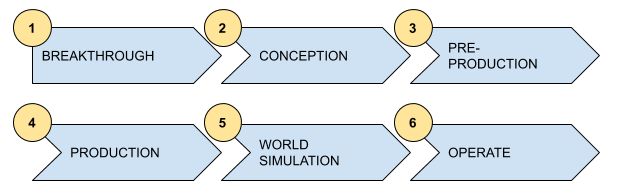
\includegraphics[width=14cm]{10_img/production_stages.png} 
    \caption{Étapes de création d'un jeu vidéo.}
    \label{fig.etapes}
\end{figure}

Les étapes de développement d'un jeu vidéo ne sont pas immuables et dépendent de l'entreprise, du domaine d'activité ou des collaborateurs impliqués dans le projet.
La figure~\ref{fig.etapes} présente une liste non exhaustive de ces étapes, telle que présentée par Mathieu Nayrolles, Architecte logiciel pour Ubisoft, lors d’un séminaire au LATECE (Laboratoire de recherche sur les Technologies du Commerce Électronique) de l’UQAM, le 10 avril 2019.



\subsection{\emph{Breakthrough}}

Une étape de \emph{Breakthrough} permet de réunir une équipe afin d'effectuer des recherches et des explorations sur des nouvelles mécaniques ou des nouvelles technologies afin de créer du nouveau contenu.
Cette étape est optionnelle dans un projet.
Deux exemples :
\begin{itemize}
    \item Une percée technologique, par ex., Google lance Stavia, une plateforme en ligne de jeux vidéos sous forme de catalogue et jouable à 100\% en ligne, sans installation en local;
    \item Une percée de \emph{gameplay}, par ex., naissance du mode \emph{Battle Royale}.
\end{itemize}

\subsection{Conception}
%Conception et non concept car c'est là que les documents sont rédigé, on parle non seulement du QUOI mais aussi du COMMENT les documents sont déjà explicites sur le COMMENT le jeu fonctionnera et sera développé

Un document de conception est défini afin d'identifier l'environnement, la faisabilité et l'intérêt commercial du jeu.
C'est durant cette étape que les \emph{Game designers} définissent et précisent l'univers, les mécaniques et le déroulement du jeu vidéo en question.
Cette étape est majoritairement gérée par les \emph{Game designers} appuyés par les équipes des autres corps de métier.
Dans des projets à financements externes, cette étape est cruciale: elle permettra de présenter le projet à un studio avec une première maquette présentant les fondements du jeu.

\subsection{Pré-production}
Durant cette étape, des prototypes sont développés afin de créer une version minimale du jeu.
Ces prototypes permettent d'avoir un aperçu jouable des concepts définis durant la phase précédente. 

Un prototype est une coupe verticale de tout le système qui permet de valider ou redéfinir les concepts.
Une fois le design bien défini, le prototype plus proche de ce que donnerait le jeu final et la faisabilité du projet confirmée, il est alors possible de rechercher les financements et les ressources nécessaires à la production.
Cette étape implique tous les corps de métier dans un studio de développement, tous les aspects du jeu devant être représentés afin de montrer tout le potentiel du prototype.

\subsection{Production}
Une fois les fonds levés et les ressources humaines attribuées au projet, il est possible de procéder à la production du jeu vidéo.
Tous les corps de métier sont représentés et le jeu est développé sous tous ses aspects et dans son intégralité.
La plupart du temps le développement est découpé en plusieurs itérations.
Chacune d'entre elles permet de vérifier que le jeu respecte bien les concepts définis plus tôt.
C'est également à ce moment que les dernières modifications sont apportées aux concepts afin qu'ils respectent la vision du \emph{Game designer} et donc génèrent la bonne expérience.
Dans le cas o\`u le projet rencontre des contraintes supplémentaires (temps, argent, plateforme, etc.), les concepts peuvent également être revus.
Généralement, durant cette étape la publicité autour du jeu commence à prendre place afin d'informer le public et afin d'estimer l'impact que pourra avoir le jeu.

\gt{Ci-haut: pas clair pour moi la distinction entre <<le marketing>> et <<la publicit\'e>>?}
              
\subsection{\emph{World simulation}}
Lors de la \emph{World simulation}, tous les éléments du jeu sont testés et passés au crible.
On vérifie que les éléments de jeu sont correctement modélisés, que les sons correspondent bien aux éléments, que les personnages correspondent à ceux décrits dans les documents de conception, etc.
Plusieurs questions se posent à cette \'etape:
\begin{itemize}
    \item Est-ce que les éléments interagissent bien entre eux ?
    \item Est-ce que l'univers de jeu est cohérent de bout en bout ?
    \item Est-ce que le \emph{gameplay} est fluide et intuitif ?
    \item Est-ce que l'environnement de jeu est réellement tel que décrit par le \emph{Game designer}?
    \item Est-ce que la bande sonore et la modélisation graphique génèrent bien les émotions attendues chez le joueur ?
\end{itemize}


\subsection{\emph{Operate}}
Le jeu est maintenant produit et commercialisé.
Une quantité importante de données est alors générée.
Des bogues peuvent être remontés et corrigés pour des cas de figure particuliers ou inédits non couverts \`a l'étape de \emph{World simulation}.
Des ajustements mineurs peuvent être faits en fonction des besoins ou des demandes des joueurs.
Le jeu prend alors toute sa dimension et toute sa vie à travers les joueurs.

Une fois le jeu bien en place et les étapes de corrections et ajustements passées, il est possible d'intégrer du nouveau contenu au jeu en repassant par les étapes précédentes.
Ce nouveau contenu est généralement intégré au jeu sous forme de mises à jours, gratuites, ou de \gls{dlc}, payants.



\section{L'exploitation vs.\ l'exploration}
\subsection{Exploitation}
Le travail \emph{d'exploitation} consiste à produire une suite à un jeu ou un nouveau jeu en utilisant des technologies (moteur, plateformes, etc.) ou un \emph{gameplay} déjà existant mais avec du contenu additionnel.
Ceci peut être fait dans le but de fidéliser une clientèle déjà existante --- en ajoutant du contenu additionnel à un jeu existant ----, d'offrir une expérience similaire avec des technologie plus récentes (par ex., FIFA) ou d'offrir une suite à un jeu ayant connu du succès (par ex., Dark Souls).

L'exploitation est une part importante du travail d'un studio de développement.
De nombreux jeux vidéos récents sont fondés sur de l'exploitation de jeux précédents, autant au niveau du \emph{gameplay} qu'au niveau des concepts fondamentaux qui sont r\'eutilis\'es de jeux précédents.
C'est le cas des (grosses) productions de franchises comme les jeux de EA sports (FIFA, NHL, NBA Live, Madden), les jeux d'action \emph{role-play} de FromSoftware (série des Dark Souls), les jeux d'action aventure de Rockstar (série des GTA) ou les jeux de simulation de Maxi/EA Games (série des Sims). 

\subsection{Exploration}
\emph{L'exploration}, ou l'innovation, dans le monde du jeu vidéo est essentielle au développement de nouveaux concepts de \emph{gameplay} mais également au développement de nouvelles technologies.
La nouveauté est un enjeu essentiel afin d'attirer toujours plus de joueurs.
L'investissement dans l'exploration est donc important pour un studio de développement.
De la recherche de nouveaux concepts de jeux, de nouveaux types de \emph{gameplay}, de nouvelles technologies à intégrer ou de la création de nouveaux moteurs de jeux, l'exploration est devenue un facteur essentiel au domaine du jeu vidéo et à son expansion.


\subsection{Équilibre entre exploitation et exploration}
Dans leur article, Parmentier \emph{et al.}~\cite{ParmentierGuy2009Iecd} explorent la capacité des studios à concilier ces deux activités.
Ils présentent les enjeux de chacune d'entre elles et leur importance dans le domaine.

Il est nécessaire pour les studios de développement de jeux vidéos de trouver le juste équilibre entre exploitation et exploration.
L'exploitation est le développement d'un jeu sur des mécanismes déjà existants où les règles sont déjà établies par un autre jeu ou un opus précédent.
L'exploration est la découverte de nouvelles mécaniques de \emph{gameplay} ou la création de nouveaux outils de développement de jeux (comme un moteur de jeu).
Le but est d'offrir aux clients des articles de qualité et attractifs.
Cet équilibre est précaire et il est difficile pour un studio de développement d'investir dans les deux domaines à la fois. 



\section{Les moteurs de jeux}
Un moteur de jeu (\emph{Game engine}) est, typiquement, une suite logicielle contenant un \emph{framework} de mécaniques de jeu --- voir Section~\ref{mechanics.sect} --- permettant d'accélérer le développement d'un jeu vidéo.
Un moteur de jeu peut inclure une ou plusieurs facettes du développement du jeu allant de la physique, aux graphismes, aux sons, aux calculs, à la gestion des périphériques d'entrée/sortie jusqu'à la gestion automatique de l'intelligence artificielle.

Voici une liste de certains des moteurs de jeu les plus connus accompagnés des jeux qui en font usage : 
\begin{itemize}
    \item \emph{Unreal Engine} (\url{https://www.unrealengine.com/}) développé par Epic Games : Fortnite, Outlast 2, Dragon Ball Fighter Z, Days Gone.
    \item \emph{Unity Engine} (\url{https://unity.com/}) développé par Unity Technologies : 7 Days to Die, Cuphead, Ori and the Blind Forest, Pokemon Go.
    \item \emph{CryEngine} (\url{https://www.cryengine.com/}) développé par Crytek : Far Cry, Crysis 3, Deceit, Mavericks.
    \item \emph{Frostbite} (\url{https://www.ea.com/frostbite}) développé par Dice (EA) : Battlefield V, Anthem, FIFA, Need for Speed.
\end{itemize}

Chaque moteur de jeu présente des avantages et des inconvénients en fonction du type de jeu que l'on souhaite développer.
Par exemple, certains moteurs sont axés sur un type de jeu ou une plateforme en particulier, et ce afin d'être plus efficaces. 
L'innovation dans les moteurs de jeu est aussi essentielle au développement de nouveaux jeux. 
Par exemple, un moteur de jeu plus récent pourra intégrer des éléments comme des graphismes plus réalistes ou détaillés, ou des intelligences artificielles plus évoluées.

\section{Les genres dans le jeu vidéo}
L'exploration peut également consister en la création d'un nouveau type de \emph{gameplay}.
Ce genre d'innovation est plus facilement identifiable par les joueurs et plus marquante en ce qui a trait \`a l'expérience de jeu.
La réunion des mécaniques de Gameplay pour réaliser un jeu complet est considérée comme un "genre" de jeux vidéos.


\gt{Ci-bas: est-ce que tu as une/des r\'ef\'erences?}

Voici une liste non exhaustive des principaux genres présents dans les jeux vidéos : (\url{https://en.wikipedia.org/wiki/List_of_video_game_genres})
\begin{itemize}
\label{MMORPG}
    \item \emph{MMORPG} (\emph{Massive Multiplayer Online Role-Playing Game}) : un jeu en ligne massivement multijoueur mettant en scène un jeu de rôle avec différents objectifs à remplir : \emph{leveling}, histoire principale vs.\ secondaire, développement social pour atteindre des objectifs sous forme de guilde, etc. (ex. : World of WarCraft, Black Desert Online).
    \item \emph{Survival} : le joueur doit survivre aux événements présents dans le jeu. Il peut devoir subvenir à des besoins vitaux, construire de nouveau objets, ou survivre aux autres joueurs présents (ex. : Rust, Ark).
    \item Plateformes : un joueur contrôle un personnage qui se déplace dans un environnement de plateformes et doit avancer tout au long du niveau pour le compl\'eter avant de pouvoir passer à un autre niveau (ex. : Mario, Donkey Kong).
    \item Simulation de vie : le joueur simule un environnement de vie plus ou moins réaliste en fonction des objectifs du jeu. La simulation peut s'appliquer à un personnage, à une ville entière, etc. (ex. : Les Sims, SimCity).
    \item FPS (\emph{First Person Shooter}) : le joueur, seul ou en équipe, doit battre des ennemis (IA ou autres joueurs) à l'aide d'armes et d'équipements de combat (ex. : Call of Duty, Halo).
    \item \emph{Beat-em up} : le joueur fait face à des vagues d'ennemis toujours plus forts (ex. : Bayonnetta, God of War).
    \item RTS (\emph{Real Time Strategy}) : des joueurs se font face dans un jeu o\`u la gestion d'économie, de troupes et de population est omniprésente afin de battre les autres joueurs (Age of Empire, Starcraft).
    \item 4X (\emph{eXplore, eXpand, eXploit, and eXterminate}) : proche du RTS, ce type de \emph{gameplay} est fondé sur une gestion pointue de ressources et de populations afin de pouvoir battre les autres joueurs sous différents aspects et avec différents objectifs de victoire (population maximale, évolution de la société, critères financiers, etc.) (ex. : Civilization, Stellaris).
    \item MOBA (\emph{Multiplayer Online Battle Arena}) : un type de \emph{gameplay} o\`u le jeu d'action rencontre le RTS. Plusieurs équipes de joueurs sont téléportées sur un territoire, chaque joueur contrôle un personnage et les joueurs doivent détruire la base de l'équipe adverse (ex. : League of Legends, DOTA).
    \item \emph{Battle Royal} : plusieurs dizaines de joueurs sont parachutés sur un territoire o\`u ils trouvent des armes et doivent s'entretuer~; le dernier survivant est déclaré vainqueur (ex. : Fortnite, PUBG/PlayerUnknown's BattleGrounds).
\end{itemize}

Les genres de jeux vidéos évoluent beaucoup.
De nouveaux genres apparaissent grâce aux recherches exploratoires.
Certains modes de jeux à succès deviennent des catégories à part entière.
Et il est possible de combiner plusieurs modes de jeu afin de créer une nouvelle expérience.
Ces divers genres de jeux vidéos sont classifiés en fonction du type de monde, des objectifs de jeu, des actions nécessaires, etc. 

Haitz et Law~\cite{HeintzStephanie2015TGGM} ont mis en place une cartographie des genres afin de classifier les différents types de jeux en se référant à des caractéristiques précises des jeux et de leur \emph{gameplay}.
Cependant, il est difficile d'arriver à classifier tous les jeux tellement les genres sont nombreux et entrecoupés.
C'est pour cela que la plupart des jeux sont classifiés dans des catégories larges et sont ensuite différenciés par leurs caractéristiques.



\section{Objectifs de notre travail de recherche}

\GT{On reverra cette section ultérieurement. Une partie de cela
devrait \^etre dans l'introduction.}

De nombreux défis entourent le développement de jeux vidéos et les outils et méthodes pour y parvenir sont variées.
Cependant, il devient de plus en plus important de chercher des méthodes afin d'accélérer le développement, sans pour autant impacter la qualité du contenu final.
Un \emph{Game designer} se doit d'être précis et concis dans ses descriptions et ses communications afin de transmettre un maximum d'informations et de pouvoir dédier plus de temps à l'exploration, à la recherche artistique et au développement d'un prototype. 



%quoi
Dans ce mémoire, nous allons présenter \gls{gg} (cf.~Section~\ref{game-genesis.sect}), un profil UML (cf.~Section~\ref{profils-UML.sect}) qui permet d'outiller le processus de pré-conception d'un jeu vidéo, facilitant ainsi la documentation et la rédaction des documents descriptifs du jeu vidéo en cours d'élaboration.

%rapidité
Destiné à être utilisé dans les premières phases du développement, \emph{Breaktrough} et Pré-conception, ce profil UML permet l'accélération de la documentation à travers un outil visuel représentant les mécaniques et les objets du jeu.
Ceci permet de produire un prototype jouable plus rapidement.

%cohérence
L'utilisation d'un profil UML permet d'apporter une structure précise et un cadre de travail rigoureux lors de la conception afin d'assurer la cohérence des modèles durant toute leur durée de vie.

%maintenance & modifications
Lors de sa conception, un jeu vidéo est destiné à évoluer rapidement et sa documentation se verra modifiée de nombreuses fois afin de toujours être la plus pertinente possible.
Le standard UML --- \gls{uml} --- permet d'apporter un support visuel à cette documentation et permet également de rendre les modifications plus faciles en accédant aux objets concernés rapidement et efficacement. 

%pérennité
Effectuer des \emph{mind mapping} est un moyen simple et efficace permettant d'illustrer des idées de manière visuelle.
Cependant, le manque de rigueur (modifications erratiques, contenu incohérents, manque de structure) et les supports utilisés (feuille de papier ou tableau) lors d'un travail de \emph{mind mapping} n'assurent pas du tout la pérennité des informations stockées.
Bien qu'il existe des logiciels de \emph{mind-mapping} qui conservent les informations sous la forme d'un fichier XML, il n'existe pas réellement de <<~standard~>> définissant de manière formelle un langage de \emph{mind-mapping}.
De plus chaque outil de \emph{mind-mapping} possède ses propres outils, ses propres méthodes et ses propres représentations.

De par sa structure imposée et précise le standard UML permet de structurer les données, de les stocker sous un format précis et de les maintenir facilement en communiquant sur les modifications effectuées.
Ceci permet un stockage beaucoup plus pérenne des informations contenues dans le modèle.

\gt{Il faudra r\'eviser ce qui pr\'ec\`ede: on peut aussi utiliser un
outil logiciel pour cr\'eation de Mind Maps, par ex., FreeMind, qui
conserve le MindMap sous forme XML.  N'en reste pas moins un
d\'esavantage: ce n'est pas un standard, i.e., chaque outil de
MindMapping a son propre format, ses propres variantes et
repr\'esentations, etc. J'ai l'impression que c'est plus de ce cot\'e
qu'il faut argumenter, que sur l'aspect papier/photos des mind maps.}


%réutilisation
UML étant un langage de modélisation largement utilisé et approuvé dans le domaine informatique, il est possible d'utiliser de nombreux outils existants, d'assurer son intégration et sa réutilisation dans différents cadres et sous différentes formes.

%gdd
Un modèle UML pourra également servir de support à la rédaction d'un \gls{gdd}, en organisant les mécaniques de jeu sous forme de catégories réutilisables.
Le GDD est la <<~bible du design~>>~\cite{GD_foundations_pedersen} du jeu.
Il permet de définir tout le contenu du jeu et toutes les informations nécessaires à son développement, et ce sur toute sa durée de vie. 

%generation de code
UML étant reconnu comme langage de modélisation de logiciels, il peut également être possible d'utiliser les modèles créés en pré-conception afin de faciliter le développement informatique du jeu.
Le modèle peut permettre de créer une structure de projet ou du pseudocode pouvant servir de squelette en début de développement.



\chapter{Les documents de \emph{Game design}}

\gt{Limiter forme <<passive>>.}

Dans ce chapitre, nous allons pr\'esenter plusieurs documents de \emph{Game design} qui sont présents dans un processus de développement de jeu vidéo. Ces documents peuvent être rédigés l'un à la suite de l'autre, ou indépendamment l'un de l'autre, et ils ne sont pas obligatoires dans chaque projet de jeu vidéo.


\gt{Je ne comprends pas <<tr\`es discut\'es>>!?}

Les documents de \emph{Game design} sont nombreux et leurs formes ainsi que leurs contenus sont souvent remis en question dans la littérature. Selon le niveau d'avancement du développement, certains sont plus utiles que d'autres mais la plupart des acteurs du domaine sont d'accord pour avancer qu'il n'existe pas de gabarit fixe pour un document de \emph{Game design}~\cite{GD_theory_rouse}. En fait, un gabarit trop sp\'ecifique et précis serait une erreur à ne pas commettre, car il pourrait entraîner des difficultés de rédaction et d'adaptation face aux divers types de jeux que l'on peut rencontrer. Cependant, certains auteurs présentent des lignes directrices, un peu comme une recette de cuisine~\cite{LevelUpRogers2014}, qui peuvent être suivies afin que le GDD soit complet et respecte une certaines forme. 

Dans sa présentation, Librande~\cite{onepage_librande} montre des exemples de livrables de game design de différentes sortes. Il souligne que les documents de design lourds sont des sources d'informations importantes, réunissant tout le design dans un seul document et la création du document aide grandement à designer le jeu par la suite. Cependant ces documents sont compliqués à maintenir, mettre à jours et à parcourir pour trouver une information précise.


\gt{Qui \c{c}a <<Il>>? Librande?}

\gt{Je ne comprends pas <<la contribution d'\'equipe>>?!}

Il présente également les <<\emph{design wikis}>> qui apportent beaucoup de points positifs au design. Il est possible d'y avoir accès à n'importe quel endroit tant qu'une connexion est disponible. Les mises à jours sont simplifiées car la recherche l'est également : il devient alors possible de modifier des éléments directement au cours d'une réunion. Un \emph{wiki} permet aussi la contribution de tous les membres de l'équipe de développement aux différents éléments car la modification est possible par de nombreux utilisateurs. Il est possible d'éditer les éléments par article et donc de ne pas avoir à prendre connaissance d'éléments non reliés au travail actuellement effectué. Il est facile de maintenir un historique des versions et des modifications pour justifier les modifications et les garder en mémoire. Cependant, un \emph{wiki} requiert une maintenance constante et donc, souvent, une personne dédiée à sa maintenance. Les relations entre les éléments ne sont pas mises en avant et il est compliqué de mettre ensemble différentes sortes de représentation sous la forme de textes/images. Autres d\'esavantages~: les images doivent être traitées à l'extérieur du \emph{wiki} avant d'y être réintégrées, et l'impression d'un article \emph{wiki} n'est pas toujours adaptée à une lecture rapide des éléments.\\
%Scott Rogers Level Up!
%Game design foundations, R. Pedersen
%Game design theory & practice Second Edition, Rouse Richard
%A Systematic Review of Game Design Methods and Tools, Gomez, Jaccheri, Hauge
%GAMASUTRA Game Design Methods: A 2003 Survey, Bernd Kreimeier 



\section{Le <<\emph{one-page}>> (ou <<\emph{one-sheet}>>): le concept document}

\gt{<<Le concept document>> ou <<La documentation des concepts du jeu>>?}



%One page designs, Stone Librante (ppt presentation)
%Game design foundations, R. Pedersen
%Scott Rogers Level Up!
Un document \emph{One page design} est une vue d'ensemble du jeu. Il est destiné à l'équipe de développement et aux acteurs décisionnels des studios. Il doit donc contenir assez d'informations à mettre en avant à propos du jeu, sauf que tout doit tenir sur une seule page~\cite{LevelUpRogers2014}.

\GT{Le premier paragraphe et le deuxi\`eme contiennent des \'el\'ements r\'ep\'etitifs, non?}

\GT{A quoi r\'ef\`ere <<ces \'el\'ements>? Pas clair!?}

C'est à partir de ces éléments que Librande~\cite{onepage_librande} estime que plus un document est long, moins les utilisateurs s'y réfèrent, et donc sa solution : le \emph{One-Page Design}.\\
L'idée est de représenter tous les éléments nécessaires au design sur une seule page et d'y intégrer toutes les informations nécessaires de manière visuelle. 

\GT{Pas clair que c'est une autre proposition --- Librande vs.\
Rogers!? A clarifier/expliciter!}


\GT{Evite d'utiliser les items de gls directement dans une phrase, car pas clair.  Apr\`es un long tiret ou entre parenth\`ese semble pr\'ef\'erable.}

\GT{Et pas n\'ecessaire d'utiliser partout, car cela alourdit le texte
--- car cela met l'item accentu\'e, ce qui ne me semble pas
appropri\'e.}

Voici les éléments que doit contenir le \emph{One-Sheet} de Rogers~\cite{LevelUpRogers2014}.
\begin{itemize}
    \item Le titre du jeu
    \item Les systèmes de jeu prévus
    \item L'age des joueurs visés
    \item La notation ESRB --- voir plus bas
    \item Un résumé de l'histoire du jeu en se concentrant sur le \emph{gameplay}
    \item Les modes du \emph{gameplay}
    \item Les USP --- voir plus bas
    \item Les produits compétitifs
\end{itemize}

\GT{Jeux et logiciels? Ou juste jeux?}

Le ESRB --- \gls{esrb} --- est un organisme d'autorégulation qui est à l'origine d'un système de notation et de règles de respect de la vie privée des jeux et logiciels. Son système de notation permet de définir à partir de points précis l'âge conseillé pour l'utilisation d'un jeu ou logiciel. C'est une notation que l'on retrouve systématiquement dans le domaine du jeu vidéo définissant le type de contenu présent dans le jeu et le public pour lequel est recommandé ce contenu : eC (\emph{Early Childhood}), E (\emph{Everyone}), E10 (\emph{Everyone~$10^+$}), T (\emph{Teen}), M (\emph{Mature} $17^+$), AO (\emph{Adults Only} $18^+$).


\GT{Est-ce vraiment des <<points>> au sens de <<pointage>>
(num\'eriques)? Ou juste des <<arguments>> --- autre sens du terme
<<point>> en anglais~: selling point = argument de vente!?}

Les USP --- \gls{usp} --- sont des points de marketing représentant le jeu. Ils se situent à l'arrière de la boite de jeu ou sur le descriptif du jeu dans le cas d'une vente dématérialisée. Ce sont des points précis et courts attirant la curiosité de l'acheteur sans être trop descriptifs. 


\GT{Je ne comprends pas le d\'ebut de la phrase suivante --- produits comp\'etitifs? Comp\'etiteurs?}

Les produits compétitifs liste les concurrents actuels du jeu, c'est-\`a-dire, ceux déjà présents sur le marché.  
Cette liste doit contenir des jeux connus ou connaissant un grand succès, afin qu'ils soient représentatifs du type du jeu d\'ecrit par le \emph{one-sheet}. Cela permet donc de donner une bonne idée de ce que le jeu sera. 
Présenter une liste de jeux obscurs ou qui n'ont connus que peu de succès découragera les éditeurs qui liront le \emph{one-sheet}.


\GT{Ci-bas: Comme c'est une liste d'\'elements, il faut que tous
soient des substantifs --- et non des actions (verbes).}

Voici les éléments essentiels d'un \emph{One-page design} tel que d\'ecrit par Librande~\cite{onepage_librande}:
\begin{itemize}
    \item Un titre représentatif du design
    \item Les dates des divers éléments, et ce afin de garder un historique
    \item Des espaces entre les informations, pour ne pas créer des blocs d'informations
    \item Une illustration centrale pour focaliser l'attention
    \item Sous l'illustration, possiblement une description et des textes explicatifs
    \item Pour des détails supplémentaires, des légendes autour de l'illustration ---
     ces légendes peuvent être des illustrations, elles-mêmes accompagnées de notes
    \item Des barres latérales pour ajouter des \emph{checklists}, des objectifs principaux ou des informations diverses
\end{itemize}

Selon Librande, la taille des éléments est importante dans un \emph{One-page design}: les tailles indiquent l'importance de l'information. Si nécessaire, un \emph{One-Page design} peut être étendu à la taille nécessaire pour contenir toute l'information, y compris sous forme d'un poster.
Cependant, l'augmentation de taille de la page doit quand même permettre d'assurer la lisibilité --- augmenter en taille ne doit pas conduire à intégrer trop d'informations, ce qui irait à l'encontre de la lisibilité.



\section{Étendre le \emph{One-page} vers un résumé}
Une fois les premières étapes de \emph{Game design} effectuées, le document \emph{One-page} va être étendu afin de produire un document plus important. Ce second document va préciser les concepts du jeu vidéo en cours de création et va permettre de communiquer un niveau de détails plus précis.

%Game design foundations, R. Pedersen
Pedersen propose le \emph{five pager}~\cite{GD_foundations_pedersen}. C'est un résumé du concept du jeu vidéo et une description du jeu à venir. Il comprend toutes les informations essentielles au cycle de vie du jeu sous ses aspects majeurs, tels que le \emph{gameplay}, l'audience cible, le scénario, et les \emph{features}. Le \emph{five-pager} permet de présenter le jeu sous sa forme la plus basique à un décideur ou à un éditeur.

\GT{Ci-haut: cela me semble contradictoire/ambigue/m\'elangeant de
dire que le document de 5 pages pr\'esente le jeu sous sa forme <<la
plus basique>>, alors qu'on a au pr\'elable produit un document d'une
seule page. Reformuler?}


\GT{Il faut \'eviter de mettre dans le corps du texte des longues
s\'eries de d\'etails tel que le contenu du \emph{Ten-pager}.  Dans le
cas pr\'esent, je crois qu'une table serait plus appropri\'ee.}


\GT{Pour une telle liste/table, pr\'ef\'erable de ne pas mettre
d'article, donc <<Titre du jeu>> plut\^ot que <<Le titre du jeu>>.  De
plus, comme \'evoqu\'e pr\'ec\'edemment, il faut \^etre uniforme,
i.e., substantifs partout --- et non pas m\'elanger substantifs et
verbes (actions).}

\begin{table}
\footnotesize
\begin{framed}
\begin{itemize}
    \item Page 1~: Informations générales
    \begin{itemize}
        \item Titre du jeu
        \item Systèmes de jeu prévus
        \item \^Age des joueurs visés
        \item Notation ESRB
        \item Calendrier prévisionnel de sortie
    \end{itemize}
    \item Page 2: Histoire
    \begin{itemize}
        \item  Résumé de l'histoire du jeu permettant de poser les premiers jalons de manière succinte et générale
        \item Résumé du déroulement du jeu  permettant de situer les actions du joueur dans l'histoire, les d\'efis rencontrés par celui-ci, comment se déroule la progression, la place du \emph{gameplay} dans l'histoire, les conditions de victoire, etc.
    \end{itemize}
    \item Page 3 : Détails du personnage contr\^ole par le joueur
    \begin{itemize}
        \item Histoire du personnage --- caractère, traits importants de son apparence
        \item \emph{Gameplay} particulier associé au personnage, ses mouvements, ses armes
        \item Maquette des contrôles proposés au joueur, par ex., représentation des raccourcis claviers
    \end{itemize}
    \item Page 4~: \emph{Gameplay}
    \begin{itemize}
        \item Modèle de séparation de l'histoire (niveaux, chapitres, monde ouvert)
        \item Scénarios particuliers (cinématique active)
        \item Mise en avant des USP
        \item Diagrammes et illustrations apportant des précisions
    \end{itemize}
    \item Page 5
    \begin{itemize}
        \item Images et description du monde du jeu
        \item Découpage des zones de jeu
        \item Liens entre les zones
    \end{itemize}

\end{itemize}
\end{framed}
\caption{Contenu du \emph{Ten-pager} selon Rogers~\cite{LevelUpRogers2014}.}
\end{table}

\addtocounter{table}{-1}

\begin{table}
\footnotesize
\begin{framed}
\begin{itemize}
    \item Page 6~: Expérience de jeu
    \begin{itemize}
        \item Description des émotions et sensations que doit générer l'expérience de jeu
        \item Description de l'interface de jeu et de la manière de les parcourir 

\GT{A quoi r\'ef\`ere <<les>> dans <<les parcourir>>? Pas clair!}

    \end{itemize}
    \item Page 7~:  Mécaniques de \emph{gameplay}
    \begin{itemize}
        \item Mécaniques : Eléments avec lequel un joueur interagit pour effectuer des actions (par ex., levier pour ouvrir une porte)
        \item Dangers : Eléments du monde pouvant tuer ou blesser le joueur mais sans IA (par ex., bloc de pierre qui tombe)
        \item \emph{Power-up} : Objets que le joueur récupère et utilise pour obtenir un avantage (par ex., champignon dans Mario)
        \item Objets de collections : Objets que le joueur collecte mais qui n'influence par directement le \emph{gameplay} (par ex.,  monnaie)
    \end{itemize}
    \item Page 8~: Ennemis
    \begin{itemize}
        \item Description des ennemis rencontrés par le joueur et qui sont contrôlés par une IA
        \item Description des \emph{boss} rencontrés
    \end{itemize}
    \item Page 9~: Multijoueur et bonus
    \begin{itemize}
        \item Description des succès collectionnables
        \item Description des secrets découvrables
        \item Description des interactions si le jeu est multijoueur
    \end{itemize}
    \item Page 10: Monétisation
    \begin{itemize}
        \item Description du système de monétisation du jeu (Gratuit, Gratuit avec une boutique en jeu, payant à l'achat, etc.)
        \item Description des boutiques et de leur contenu
    \end{itemize}
\end{itemize}
\end{framed}
\caption{Contenu du \emph{Ten-pager} selon Rogers~\cite{LevelUpRogers2014} (suite).}
\label{ten-pager.table}
\end{table}

Quant \`a Rogers~\cite{LevelUpRogers2014}, il  propose un document plus \emph{fourni} avec son \emph{Ten-pager}. Ce document comporte deux parties, qui se différencient radicalement en fonction du destinataire. Le contenu du document doit non seulement contenir des informations pour l'équipe de développement du jeu, mais également les informations nécessaires pour int\'eresser les éditeurs impliqués dans le projet. Rogers présente le contenu du \emph{Ten-pager} sous la forme suivante indiqu\'ee dans le tableau~\ref{ten-pager.table}.
%
\ACOMPLETER{Alors que les pages X \`a Y sont destin\'ees plus
sp\'ecifiquement \`a Z, les pages U \`a V sont destin\'ees \`a W.}
    
\GT{Paragraphe ci-haut~:  Tu parles de deux parties avec destinataires distincts. Ce serait bien d'expliciter}




\section{Le \emph{Game Design Document}}
%Game design foundations, R. Pedersen
%Proposal of Game Design Document from Software Engineering Requirements Perspective, Mario Gonzalez Salazar, Hugo A. Mitre, Cuauhtémoc Lemus Olalde, José Luis González Sánchez

%Incorporating a Game Design Document into Game Development Projects Deliverables,Craig Marais,Lynn Futcher,Johan van Niekerk
%GAMASUTRA Creating a great design document Tzvi Freeman

%Improving Game Development Process Applying Multi-View Game Design Documents,Pablo Correa , Luisa Möller 
%6


%GAMASUTRA 5 Alternatives to a Game Design Document, Erin Robinson

\subsection{Le GDD, un moyen de communication}
Le \gls{gdd} est un des documents les plus complet trouvable dans le cadre du développement d'un jeu vidéo. Dans la littérature il est souvent qualifié de <<Bible du design>>~\cite{GD_foundations_pedersen} --- bien que certains auteurs ne soient pas d'accord sur ce sujet~\cite{LevelUpRogers2014}. 

Le GDD doit contenir, dans l'idéal, toute la vision du \emph{game designer} sans laisser de doute sur ce que celui-ci veut représenter et souhaite voir dans le jeu. Peu importe le corps de métier de la personne lisant le GDD, celle-ci doit pouvoir se représenter au maximum le rendu final attendu. Le GDD doit donc pouvoir servir de moyen communication entre les différentes équipes entourant le développement du jeu, et ce \`a toutes les étapes, depuis la création de l'idée jusqu'au post-mortem du projet.

\subsection{Une structure souple mais un contenu précis}

\GT{Lorsqu'on indique un auteur, il suffit de mettre le nom de famille, sans le pr\'enom.}

Dans un article sur Gamasutra~\cite{gama_greateGDD}, Freeman établit une liste de 10 pratiques qu'il estime nécessaire de respecter pour d\'ecrire un GDD :
\begin{itemize}
    \item Décrire le corps du jeu, mais également son âme
    \item Rendre le GDD lisible
    \item Etablir des priorité dans les tâches
    \item Rentrer au maximum dans les détails
    \item Démontrer et décrire les sujets
    \item Décrire le <<quoi>> mais également le <<comment>>
    \item Proposer des alternatives sur certaines réalisations \GT{Pas clair: des alternatives de mises en oeuvres?}
    \item Donner une vie au GDD
    \item Pr\'eciser la vision du \emph{Game designer} de fa\c{c}on suffisamment précise pour ne pas laisser d'éléments non décrits
    \item Mettre à disposition le GDD dans de bonnes conditions
\end{itemize}

\subsection{Un GDD complet mais pas surchargé}

\GT{Ci-bas~: j'ai reformul\'e la premi\`ere phrase car c'\'etait vague
de parler <<d'outils>> et c'\'etait bizarre de m\'elanger outils et
libert\'e: A revoir!}

Le GDD doit \^etre un outil pour les \emph{game designers}, tout en leur donnant la liberté de créer de nouveaux jeux, de nouveaux \emph{gameplay}, de nouveaux concepts, donc sans les brider dans leur cr\'eativit\'e. De nombreux travaux essaient de répondre au besoin de formalisation du GDD~\cite{GDD_software,multiview,GDD_GDProject,gama_greateGDD} sans pour autant réussir à apporter une solution permettant d'englober tous les types de jeux, tous les types de métiers ou toutes les étapes de développement. Et de nombreux problèmes annexes se posent concernant l'universalité d'un modèle de GDD : Est-il complet ? Est-il assez précis ? Est-il assez souple ? Est-il utile à l'équipe ? 

Prenons l'exemple d'un projet où le GDD est extrêmement complet, comportant tous les détails voulus par le \emph{Game designer}. Le GDD peut alors devenir tellement complet qu'il en devient imposant, lourd à parcourir, difficile à maintenir et à modifier. Il perdra alors toute l'efficacité de design qu'il aurait pu donner, pouvant devenir un handicap de temps plutôt qu'une aide au développement~\cite{onepage_librande}.

Un GDD est l'atout majeur de la phase de production d'un jeu vidéo et pour qu'il soit utile durant toutes les phases celui-ci doit être impérativement complet et sans ambiguité~\cite{GD_Guidelines}. Cependant il doit être assez souple afin de suivre le jeu dans son développement et suivre les changements nombreux et soudains qui peuvent arriver au cours du développement.

Dans son article~\cite{gama_greateGDD}, Freeman écrit que le GDD doit non seulement décrire le corps du jeu vidéo mais son <<âme>>. Construire un GDD selon lui doit être un moyen de représenter le résultat attendu dans les moindres détails pour permettre aux équipes de travailler sur une idée précise. Faire appel à des outils graphiques plutôt qu'à des textes peut être un moyen d'apporter plus de précision à une idée. Mais le GDD doit être un moyen d'expliquer toutes les parties du jeu, le <<quoi>>, mais également le <<comment>>.

Cependant décrire l'intégralité des détails dans le GDD peut mener à des dérives décrites par Rouse~\cite{GD_theory_rouse}. À vouloir apporter trop de détails dans un GDD, un \emph{Game designer} peut perdre énormément de temps qui aurait pu être économisé avec plus de communication avec son équipe. Trop de détails peut également apporter trop de limitations aux corps de métier plus artistiques et brider leur créativité. Certaines parties du jeu peuvent également en obstruer d'autres : trop de détails dans la description d'une mécanique peut éclipser le fait qu'une autre n'est pas assez détaillée. Un GDD trop complet donne également l'impression que le projet est terminé et qu'il ne nécessite plus d'ajustements, cela nuit à l'évolution du jeu et aux modifications positives qui pourraient lui être appliquées.


\GT{Il va falloir que je relise cette derni\`ere section --- en fait,
le chapitre au complet --- car j'ai l'impression qu'il y a certaines
redondances/r\'ep\'etitions, mais aussi quelques aspects manquants
dans le fil logique.}



\section{Conclusion}
Dans ce chapitre, nous avons vu quatre sortes de documents de \emph{Game design}~: \ACOMPLETER{Les nommer ici, comme rappel/r\'esum\'e/synth\`ese}.
%  
Ces documents sont les plus répandus dans le monde du développement de jeux vidéos. 

Selon le type de \emph{gameplay}, la quantité d'informations ou la durée de vie du jeu, un GDD peut avoir une taille plus ou moins importante. 
%
La structure du GDD peut différer d'un \emph{Game designer} à l'autre en fonction des habitudes de travail avec son équipe ou son expérience. Le contenu du GDD peut aussi être sous formes diverses :  textes,  graphiques, diagrammes,  \emph{mind mapps}. 

C'est pour ces raisons qu'il est compliqué d'établir un gabarit précis pour la rédaction d'un GDD. La structure de tels documents n'est pas fixe et leur rédaction peut \^etre effectuée en suivant des bonnes pratiques décrites par des \emph{Game designer} expérimentés et trouvent réellement leur forme par la manière dont un \emph{Game designer} souhaite partager sa vision du futur jeu.

\GT{Derni\`ere phrase \`a relire!!!}

\chapter{Le \emph{framework} <<\emph{Mechanics}, \emph{Dynamics}, \emph{Aesthetics}>> (MDA)}
\label{chap.MDA}

\gt{Pas trop clair le d\'ebut!?}

La conception de jeux est le processus de réflexion nécessaire à la création d'un jeu.
C'est l'évolution que subit le jeu depuis une idée initiale jusqu'à sa réalisation finale.
De nombreuses étapes permettent de modéliser et formaliser tous les aspects du jeu pour le mener à sa version jouable : 
la mise en place du cadre spatio-temporel dans lequel le joueur évoluera, les règles qu'il devra suivre pour avancer, les éléments graphiques qu'il rencontrera. Tout cela est défini lors de la conception. 

Un jeu vidéo est cependant difficile à concevoir et, surtout, à documenter.
Un logiciel classique vise généralement \`a répondre à un besoin précis identifié et demandé par les utilisateurs.
Le logiciel est donc une réponse à une problématique et son utilisation est logique si le logiciel répond au besoin énoncé.
%
Par contre, un jeu vidéo doit créer le besoin chez un utilisateur, qui n'a pas de besoins liés à son utilisation.
Il doit proposer un but au joueur, lui donner l'envie de continuer à l'utiliser et doit générer des émotions pour être apprécié, car il ne vise pas \`a r\'esoudre une problématique.

Il est compliqué de définir une méthode précise pour décrire une émotion ainsi que les moyens à mettre en place pour parvenir à la générer.
Le \emph{framework} \glsfirst{mda} tente de définir une structure pour accompagner un \emph{game designer} durant les étapes de documentation d'un jeu.
MDA essaie d'apporter une solution en apportant une catégorisation des émotions et des approches et techniques pour parvenir à les générer.


\section{Le jeu : un échange entre \emph{game designer} et joueur}


\gt{Ne pas oublier: mettre un espace ins\'ecable --- tilde --- avant cite et avant ref!}


\begin{figure}
    \begin{center}
    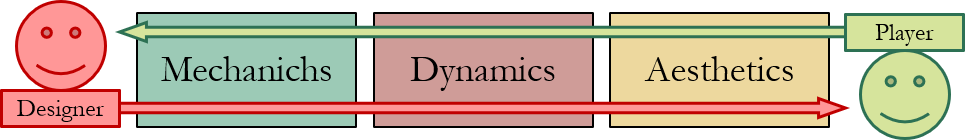
\includegraphics[width=14cm]{10_img/chap3/mda.png} 
    \caption{Les trois parties du \emph{framework} MDA~\cite{MDA_formal}.}
    \label{fig:mda}
    \end{center}
\end{figure}

Un \emph{game designer} cr\'ee un jeu dans le but de générer une expérience de jeu. 
Cependant, l'utilisation que le joueur fera du produit fini est difficile \`a pr\'evoir, comme
le d\'ecrivent Hunicke, LeBlanc et Zubek~\cite{MDA_formal}, qui découpent un jeu en trois aspects distincts : les règles, le système et le <<~fun~>>. 
Ces trois aspects sont à l'origine des trois parties du \emph{framework} MDA, tel qu'illustré dans la Figure~\ref{fig:mda}, que nous expliquons plus en d\'etail dans les sections qui suivent.


%MDA: A Formal Approach to Game Design and Game Research Robin Hunicke, Marc LeBlanc, Robert Zubek
%A better recipe for game jams: using the Mechanics Dynamics Aesthetics framework for planning Paris Buttfield-Addison,Jon Manning,Tim Nugent
%\Design, Dynamics, Experience (DDE): An Advancement of the MDA Framework for Game Design
\section{\emph{Mechanics}}

\label{mechanics.sect}

\gt{Malgr\'e le <<s>> final, <<mechanics>> est singulier --- comme la
m\'ecanique quantique.  Au singulier, <<mechanic>> d\'enote un
m\'ecanicien~:
\url{https://www.merriam-webster.com/dictionary/dynamics}. Idem pour
les autres aspects de MDA.}

\gt{Je ne comprends pas la 2e phrase, qui ne dit pas grand chose je
trouve: <<Les \'elements [\ldots[ plus pr\'ecis\'ement. J'ai tent\'e de reformuler.}

L'aspect \emph{Mechanics} d'un jeu est compos\'e de tous les éléments du jeu associ\'es \`a la représentation des données et des algorithmes. 
Les éléments de \emph{Mechanics} sont class\'es en diverses catégories, qui permettent de les définir plus précisément. 
Ces catégories peuvent comprendre des attributs et des spécificités qui sont appliquées aux divers éléments de chaque catégorie.

La \emph{Mechanics} comprend également les actions, comportements et mécanismes de contrôles mis à disposition du joueur. 
Cela peut correspondre aux mouvements d'un personnages, aux actions possibles sur des objets ou aux interactions entre les objets. Les règles sont aussi définies dans les mécaniques.


\section{\emph{Dynamics}}

Les \'el\'ements de l'aspect \emph{Dynamics} repr\'esentent les conséquences des \'el\'ements de \emph{Mechanics}. 
Ils décrivent le comportement de l'exécution de la \emph{Mechanics}, lorsqu'ils seront effectivement utilisées par le joueur~\cite{GAMA_MDA}. 
Ces \'el\'ements de \emph{Dynamics} sont importants à prévoir car ce sont eux qui permettront l'évolution du joueur dans le jeu.

Afin de définir la \emph{Dynamics}, il est possible d'analyser d'autres jeux (de même genre ou d'opus précédents); il est aussi possible d'effectuer des analyses statistiques sur les habitudes de jeu des joueurs, d'étudier leur psychologie afin de prévoir leur \emph{gameplay} et en jouant sur leurs émotions.


\section{\emph{Aesthetics}}
Les \'el\'ements de l'aspect \emph{Aesthetics} sont, selon Hunicke, LeBlanc et Zubek~\cite{MDA_formal}, <<~ce qui rend le jeu \emph{<<fun>>}~>>. 
Ce sont toutes les émotions générées par le jeu et transmises au joueur par l'interm\'ediaire de la mécanique de jeu, des sons ou des graphismes. Hunicke, Leblanc et Zubek classifient ces \'el\'ements en huit catégories :
\begin{itemize}
    \item Sensation : le jeu comme plaisir des sens.
    \item Fantaisie : le jeu comme imaginaire.
    \item Narration : le jeu comme situation dramatique.
    \item D\'efi : le jeu comme parcours d'obstacles.
    \item Communauté : le jeu comme réseau social.
    \item Découverte : le jeu comme territoire inexploré.
    \item Expression : le jeu comme découverte de soi-même.
    \item Soumission : le jeu comme passe-temps.
\end{itemize}

\gt{Les tildes (espaces ins\'ecables) sont important si tu utilises
guilletmotleft/right! Je trouve plus simple d'utiliser <<...>>, ce qui
donne la m\^eme chose sur ma machine. Et sur Overleaf, \c{c}a donne le
bon r\'esultat ou pas?}

Le jeu final peut contenir une ou plusieurs catégories de <<fun>> et l'ensemble de l'expérience du joueur repose sur ces \'el\'ements d'\emph{Aesthetics}. 
Cette dernière partie du \emph{game design} est si importante qu'il est possible de concevoir et développer le jeu en ayant au préalable sélectionné un certain nombre de ces catégories et en les considérant comme objectifs à atteindre.




\section{Des évolutions du \emph{framework} MDA}

Le MDA permet de modéliser la conception du jeu vidéo en séparant trois aspects cl\'es d'un jeu : les éléments de \emph{Mechanics}, de \emph{Dynamics} et d'\emph{Aesthetics}.
Cependant, de nombreux auteurs critiquent MDA car certains genres de jeu ou certaines mécaniques de \emph{gameplay} sont exclus de ce \emph{framework}.
%
D'autres \emph{frameworks} ont donc été proposés.
%
Par exemple, les \emph{frameworks} <<~\emph{Design, Play, Experience}~>> (DPE) (Sect.~\ref{sect.MDA_DPE}) --- qui cherche à intégrer les jeux reposant uniquement sur l'histoire, les jeux sérieux ou les outils d'apprentissage ludique ---
%
et <<~\emph{Design, Dynamics, Experience}~>> (DDE) (Sect.~\ref{sect.MDA_DDE}) --- qui avance que MDA néglige certains aspects du design de jeux vidéos en se concentrant trop sur les éléments de \emph{Mechanics}.

\gt{En quelques mots, en guise <<d'introduction>> \`a cette
section, il faudrait indiquer certaines limitation de MDA, pour
motiver pourquoi d'autres frameworks ont \'et\'e propos\'es.}


\subsection{Le \emph{framework} <<\emph{Design, Play, Experience}>> (DPE)}
%ARTCILE The Design, Play, and Experience Framework, Brian M. Winn
\label{sect.MDA_DPE}

\begin{figure}[H]
    \centering
    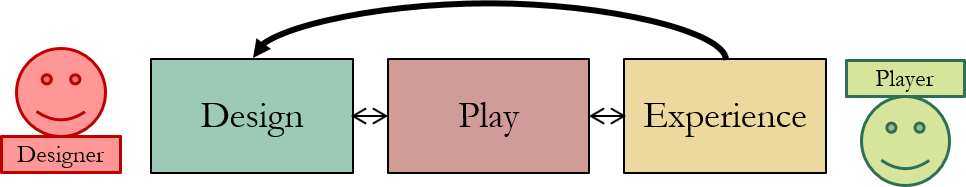
\includegraphics[width=10cm]{10_img/chap3/dpe.png} 
    \caption{Les trois parties du \emph{framework} DPE~\cite{Winn2011}.}
    \label{fig.dpe}
\end{figure}

Le \gls{dpe}, illustr\'e \`a la figure~\ref{fig.dpe}, est un \emph{framework} reposant sur les mêmes principes que MDA. 
Plus sp\'ecifiquement, des modifications sont appliquées au MDA afin d'étendre ses capacités de design pour les jeux sérieux. 
Ainsi, DPE étend MDA afin d'y intégrer les notions d'apprentissage, de \emph{story telling}, de \emph{gameplay} et de composants technologiques spécifiques aux jeux sérieux. 
La figure~\ref{fig.dpe_extended} donne les différentes parties du DPE, telles que présentées par Winn~\cite{Winn2011}.


\begin{figure}
    \centering
    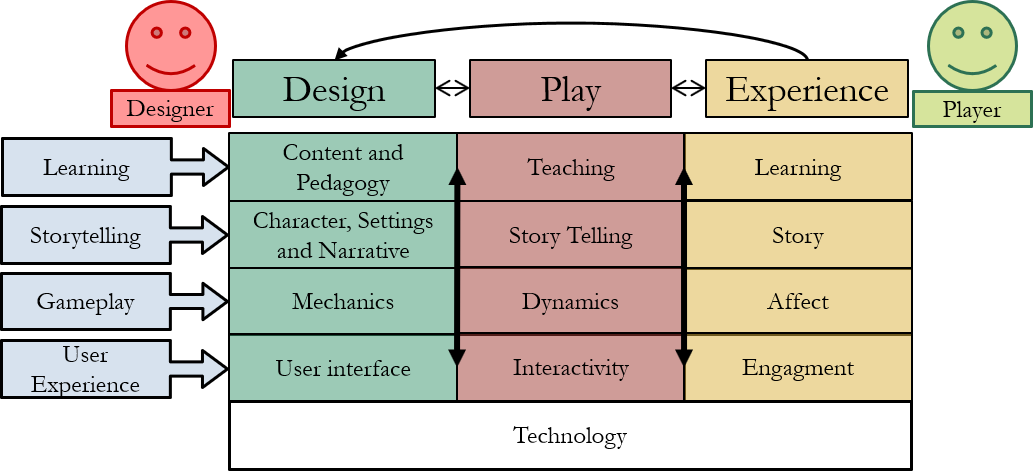
\includegraphics[width=14cm]{10_img/chap3/dpe_extended.png} 
    \caption{Les d\'etails du \emph{framework} DPE~\cite{Winn2011}.}
    \label{fig.dpe_extended}
\end{figure}


\begin{figure}
    \centering
    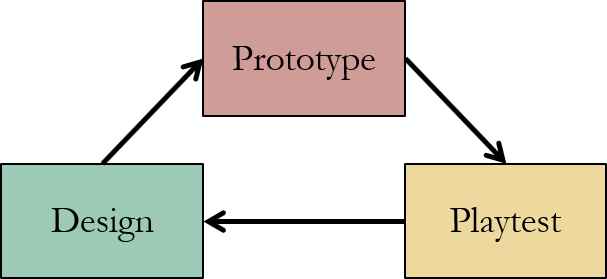
\includegraphics[width=8cm]{10_img/chap3/iteration_prototype.png} 
    \caption{Le processus de design itératif associ\'e \`a DPE~\cite{Winn2011}.}
    \label{fig.dpe_iteratif}
\end{figure}


Dans le \emph{framework} DPE, le \emph{game designer} a le contrôle direct sur l'ensemble des catégories. 
Notamment, le \emph{game designer} définit explicitement des objectifs d'\emph{Experience}. 
C'est ce qui est représenté, dans la figure~\ref{fig.dpe_extended}, par la flèche entre allant d'\emph{Experience} vers \emph{Design}. 
Cette flèche représente également le processus itératif du design décrit par Salen et Zimmermann~\cite{Salen2013}, tel qu'illustr\'e \`a la figure~\ref{fig.dpe_iteratif}. 
La conception permet de produire un prototype, et l'expérience sur ce prototype permet de modifier le design afin que l'\emph{Experience} corresponde aux attentes du \emph{game designer}.




\subsection{Le \emph{framework} <<~\emph{Design, Dynamics, Experience}~>> (DDE)}
\label{sect.MDA_DDE}
%ARTICLE DDE Design, Dynamics, Experience (DDE): An Advancement of the MDA framework for Game Design Wolfgang

\begin{figure}
    \begin{center}
    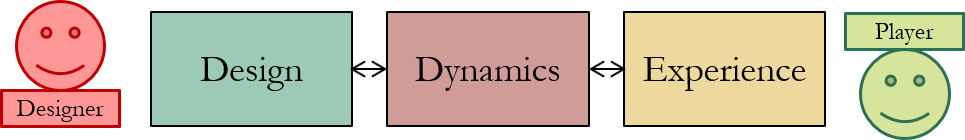
\includegraphics[width=10cm]{10_img/chap3/dde.png} 
    \caption{Les \'el\'ements du \emph{framework} DDE~\cite{DDE}.}
    \label{fig.dde}
    \end{center}
\end{figure}

\begin{figure}
    \begin{center}
    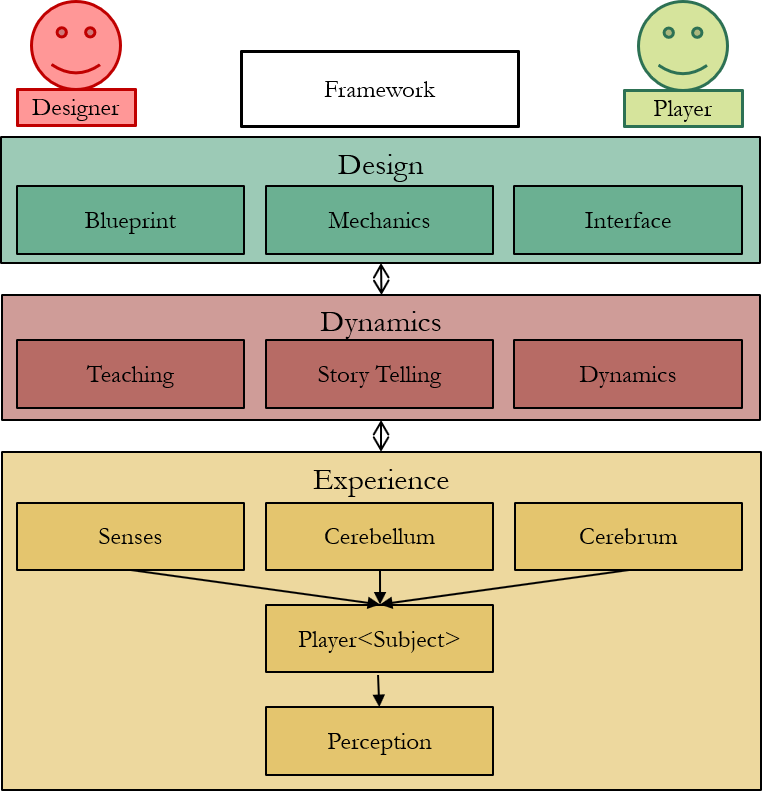
\includegraphics[width=13cm]{10_img/chap3/dde_extended_modif.png} 
    \caption{Les d\'etails du \emph{framework} DDE~\cite{DDE}.}
    \label{fig.dde_extended}
    \end{center}
\end{figure}

%GAMASUTRA From MDA to DDE, Wolfgang Walk
Le framework \gls{dde}, illustr\'e \`a la figure~\ref{fig.dde}, a \'et\'e propos\'e par Walk \emph{et~al.}~\cite{DDE}. 
Ils apportent une vision critique du \emph{framework} MDA et avancent que celui-ci néglige de nombreux aspects du design de jeux vidéos. 
Ils estiment également que MDA se concentre trop sur l'aspect \emph{Mechanics} et ne permet donc pas de décrire tous les types de \emph{gameplay} présents sur le marché. 
Ce focus sur l'aspect \emph{Mechanics} entraîne, selon Walk \emph{et~al.}, un manque de contrôle du \emph{game designer} sur les aspect \emph{Dynamics} et \emph{Aesthetics} qui ne font que découler de l'aspect \emph{Mechanics}
%
Walk \emph{et al.} effectuent donc un découpage différent et intègrent de nouvelles notions dans les catégories, tel qu'illustr\'e dans la figure~\ref{fig.dde_extended}.




\GT{J'ai mis des sous-sections non-numérotées, sinon c'est trop
profond comme numérotation et ça rend cela débalancé par rapport aux
autres sous-sections.}

\subsubsection*{\emph{Design}}

Les \'el\'ements associ\'es \`a l'aspect \emph{Design} sont les suivants~: 
    \begin{itemize}
\item \emph{Blueprint} : Partie du design qui concerne les concepts du monde du jeu : culture, religion, physique, ensembles de règles, styles artistiques, design narratif, design de personnages et design sonore, qui ensemble créent l'expérience esthétique.
\item \emph{Mechanics} : Toute chose créant le jeu, plus précisément le code. L'architecture du code, la prise en charge des entrées/sorties, la prise en charge des objets, l'implémentation des règles de jeu et l'interaction entre les objets, et tous les éléments reliés au code. Cela comprend donc tous les éléments que le joueur ne perçoit pas directement dans son utilisation du jeu.
\item Interface : Toutes les mécaniques qui ont pour but
    de communiquer le jeu au joueur. Les graphismes, les sons, les
    réactions et les interactions. Ces mécaniques peuvent aussi servir
    à effectuer une communication sous la forme
    Jeu~$\Rightarrow$~Joueur, Joueur~$\Rightarrow$~Jeu ou
    Jeu~$\Rightarrow$~Jeu. Cette partie comprend également les
    cinématiques, les textes affichés, et tout ce qu'il est possible
    de voir ou d'entendre dans le jeu.
\end{itemize}
%
\subsubsection*{\emph{Dynamics}} 

La catégorie \emph{Dynamics} de DDE correspond à celle de MDA, mais elle classifie les interactions de manière à les rendre plus précises, d\'ecompos\'ees en trois sous-catégories: 


    \begin{itemize}
        \item \emph{Player} $\Leftrightarrow$ \emph{Game}
        \item \emph{Player} $\Leftrightarrow$ \emph{Player}
        \item \emph{Game} $\Leftrightarrow$ \emph{Game}
    \end{itemize}

\subsubsection*{\emph{Experience}}
    Dans le \emph{framework} MDA, la troisième partie est l'\emph{Aesthetics} : tout ce que le joueur sent et ressent lors de son activité et interaction avec le jeu. 
    La partie \emph{Exprience} du jeu étend l'\emph{Aesthetics} afin de prendre en considération que le joueur n'est pas uniquement la somme des émotions générées par le jeu. 
    Le joueur devient un élément avec une expérience déjà présente avant l'utilisation du jeu, ce qui peut modifier les émotions générées d'un joueur à l'autre. Une même couleur, un même son ou une même image peuvent générer différentes réactions de la part du joueur et la partie \emph{Experience} de DDE essaie de prendre cela en compte.
    \begin{itemize}
        \item \emph{Senses}: expérience sensorielle du joueur du début à la fin du jeu.
        \item \emph{Cerebellum} : les émotions ressenties par le joueur.
        \item \emph{Cerebrum} : les d\'efis intellectuels et les décisions prises par le joueur.
        \item \emph{Player<Subject>} : la partie que le designer ne peut pas contrôler. Il peut se baser sur les trois premières catégories afin de prévoir certaines réponses spécifiques du joueur. N'ayant aucun contrôle sur celles-ci, le designer ne peut qu'estimer la réaction du joueur en fonction d'objectifs et de logiques psychologiques pour l'amener à la réaction souhaitée.
        \item \emph{Perception} : ce que ressent réellement le joueur en fonction des trois premières catégories et de sa propre expérience et personnalité en tant que joueur. Cela comprendra son \emph{gameplay}, le type de d\'efi qu'il perçoit, l'amusement qu'il ressent, la beauté qu'il perçoit, l'écho que génère l'histoire en lui, etc.
    \end{itemize}


%GAMASUTRA Revisiting the MDA framework, Luiz Claudio Silveira Duarte
\subsection{Une autre limite du \emph{framework} MDA}
Dans une critique du \emph{framework} MDA, Duarte~\cite{GAMA_MDA} met de l'avant les difficultés  rencontr\'ees à représenter, \`a l'aide de MDA, des jeux qui ne soient pas des jeux vidéos. 
Duarte explique que les règles d'un jeu vidéo sont souvent implicites au type de \emph{gameplay} ou genre de jeu vidéos. 
Cependant, dans le cadre des jeux de plateau, les règles ne peuvent pas être implicites et acquises par l'expérience. 
Elles doivent être explicites et explicables dans un manuel d'utilisation. 
Il fait l'analogie entre un jeu FPS --- \gls{fps} --- et un jeu d'échecs. Dans un FPS, un joueur sait à quoi s'attendre en fonction de son expérience du genre du jeu. 
Il saura o\`u trouver les éléments et saura comment faire usage de l'interface graphique qui lui est présentée. 
Cependant, un joueur se trouvant devant un jeu d'échecs pour la première fois ne pourra pas acquérir par l'exp\'erience les connaissances requises pour jouer~: les règles devront lui être expliquées à la base et l'expérience pourra lui apporter des aspects tactiques ou strat\'egiques du jeu.

\section{Conclusion}

\ACOMPLETER{Ta conclusion devra donc <<mettre la table>> pour ce qui
s'en vient dans le chapitre V, à savoir que tu vas te concentrer sur
l'aspect M de MDA, car c'est le socle sur lequel tout repose ---
puisque ça définit le <<modèle conceptuel>> du jeu!}

\chapter{Les profils UML}
%OMG Unified Modeling LanguageTM (OMG UML),Superstructure
\label{chap.profils-UML}
\section{Le langage de modélisation UML}

Le \glsfirst{uml} est un langage de modélisation standardisé permettant de créer des mod\`eles, typiquement sous forme de diagrammes.
Ces diagrammes permettent de visualiser, spécifier, construire et documenter des logiciels, des systèmes et des processus d'affaire.
UML utilise diverses notations,  surtout graphiques, pour exprimer l'architecture, le design ainsi que la mise en \oe{}uvre de logiciels.
Les spécifications du standard UML sont en ligne sur le site de l'OMG (\emph{Object Management Group})~\cite{OMG_UML}.

\gt{Comme indiqu\'e pr\'ec\'emment, sauf certaines exceptions, on
n'utilise pas trop le positionnement [H], i.e., on laisse flotter, on
laisse \LaTeX\ d\'ecider o\`u mettre la figure. Par contre, on met les
figures ou tableaux *avant* la r\'ef\'erence.}


\gt{Dans la figure 4.1: Tu indiques <<Diagrammes structurels>> mais
dans le texte tu parles de <<Diagrammes de structure>>.  Et ce serait
mieux de mettre au singulier aussi, car les autres boites sont au
singulier. Et <<de \underline{de} structures composites>>!}

\gt{Figure 4.2: Idem: parfois Diagrammes, parfois Diagramme. Mettre
singulier partout.}
 
\begin{figure}
    \centering
    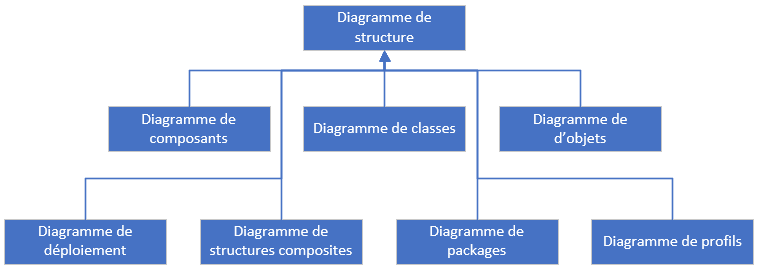
\includegraphics[width=12cm]{10_img/chap4/structure.PNG}
    \caption{Les principaux types de diagrammes de structure d'UML~\cite{OMG_UML}.}
    \label{fig.uml_struc}
\end{figure}

\begin{figure}
    \centering
    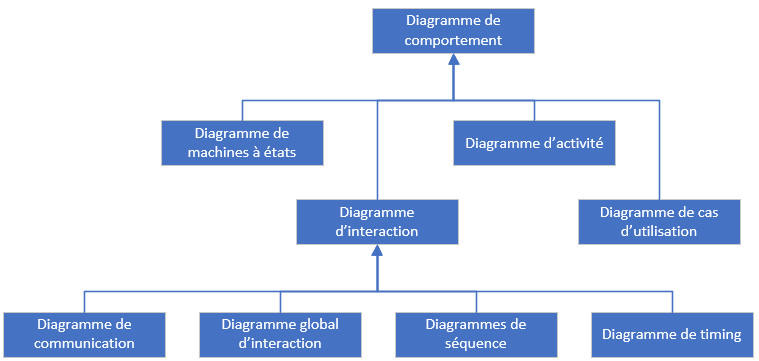
\includegraphics[width=12cm]{10_img/chap4/comportement.PNG}
    \caption{Les principaux types de diagrammes de comportement d'UML~\cite{OMG_UML}.}
    \label{fig.uml_comp}
\end{figure}


\gt{Il vaut mieux utiliser une forme <<active>> --- <<La figure
pr\'esente>> --- qu'une forme passive --- <<Dans la figure sont
pr\'esent\'es\ldots>>.}

La figure~\ref{fig.uml_struc} présente les principaux types de diagrammes de structure proposés par UML,
alors que la figure~\ref{fig.uml_comp} présente les principaux types de diagrammes de comportement.

UML \'etant un langage de modélisation largement connu et bien documenté dans le domaine du g\'enie logiciel,
nous nous concentrons dans le pr\'esent chapitre plus particulièrement à définir les notions nécessaires à la compréhension des mécanismes et des éléments composant les profils UML.



\section{La notion de profil en UML}

\gt{UML pr\'esente diverses notions, qui peuvent \^etre
repr\'esent\'ees de fa\c{c}on graphique ou textuelle.  Donc, en soit,
aucun item UML n'est un diagramme.  Le diagramme est une des
repr\'esentations possibles d'une notion.}


Un profil UML est un m\'ecanisme d'extension, qui
permet d'étendre les éléments d'UML afin d'adapter les mod\`eles et leur contenu à un domaine particulier (par ex.,  domaines d'activité spécifique) ou \`a une plateforme particulière (par ex.,  .NET, J2EE).

Les extensions qu'un profil d\'efinit permettent d'ajouter des caractéristiques aux éléments standards d'UML.
Ces extensions ne peuvent pas \emph{retirer} des caractéristiques, et ce pour ne pas aller à l'encontre de la sémantique standard d'UML.
Un profil se compose  de stéréotypes, de valeurs \'etiquet\'ees (\emph{tagged values}) et de contraintes qui s'appliquent aux éléments de modèles UML tels que les classes, les attributs, les opérations et les activités.

\gt{Pour l'exemple, pas une bonne idée d'avoir une sous-section
numérotée --- parce qu'alors, il y a une seule sous-section numérotée,
ce qui n'est pas d'un bon style.}

\subsection*{Exemple}
%
Afin de mieux comprendre les éléments qui composent un profil, nous allons mettre en place un exemple au fur et à mesure de ce chapitre, en y intégrant divers éléments un \`a la fois.

\begin{figure}
    \centering
    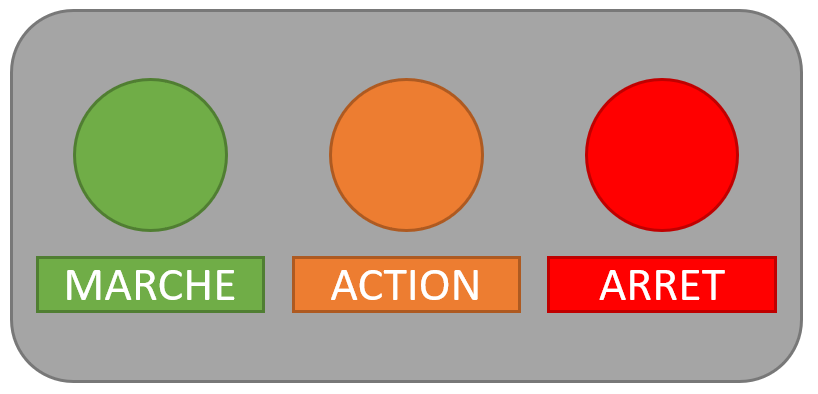
\includegraphics[width=8cm]{10_img/chap4/example.PNG}
    \caption{Le tableau de bord de la machine pour notre exemple de profil UML.}
    \label{fig.uml_ex}
\end{figure}

Prenons un exemple d'un mod\`ele devant représenter un tableau de bord d'une machine composée de trois boutons : \texttt{Marche}, \texttt{Action}, \texttt{Arrêt}.
Chaque bouton a un état <<\texttt{actif}>> ou <<\texttt{inactif}>>, et
chacun a une action qui lui est propre sur la machine contr\^ol\'ee par ces boutons : \texttt{Marche} = démarre la machine; \texttt{Action} = effectue l'action de la machine; \texttt{Arrêt} = termine l'ex\'ecution de la machine.
%
La figure~\ref{fig.uml_ex} illustre un tableau de bord possible pour une telle machine.

%\newpage \GT{A EVITER, sauf a la toute fin, quand on veut fignoler la mise en page!}

\section{Les stéréotypes}
\label{sect.uml.ster}
Les stéréotypes permettent de spécifier des extensions aux métaclasses UML.
Ceci permet d'ajouter des termes spécifiques de vocabulaire à un mod\`ele.
Un stéréotype peut être défini pour divers types d'éléments d'un mod\`ele UML, par exemple, classes, associations, attributs, etc.


\subsection*{Exemple}
%
\begin{figure}
    \begin{center}
    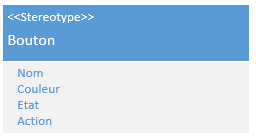
\includegraphics[width=6cm]{10_img/chap4/button.PNG}
    \caption{Un st\'er\'eotype <<\texttt{Bouton}>> permettant de sp\'ecifier les points communs aux diff\'erents boutons.}
    \label{fig.uml_but_definition}
    \end{center}
\end{figure}

Dans la figure~\ref{fig.uml_but_definition}, on remarque la présence d'une flèche noire à tête pleine entre les éléments "\texttt{<<stereotype>> Bouton}" et "\texttt{<<metaclass>>~Class}".
C'est la notation (graphique) UML indiquant que le st\'er\'eotype \texttt{Bouton} \textbf{étend} (\emph{extension}) la métaclasse UML \texttt{Class}.
%
En d'autres mots, le stéréotype \texttt{Bouton} pourra être utilisé pour \emph{annoter des classes.}
%
Signalons aussi qu'une extension, comme on le verra dans le prochain chapitre, peut aussi être utilisée en lien avec la métaclasse \texttt{Association}, ce qui permet alors de stéréotyper une association.

\begin{comment}
\GT{Pas nécessaire... et pas certain pour la multiplicité!?}

La notation d'extension peut inclure différents éléments, mais qui ne sont pas requis dans notre cas comme :
\begin{itemize}
    \item la notation \emph{<<~required~>>} qui indiquerait que l'extension est obligatoire sur chaque élément de \texttt{<<~metaclass~>>Class}.
    \item des multiplicités qui définissent si un objet \texttt{<<~metaclass~>>Class} peut être étendu par un ou plusieurs stéréotypes.
\end{itemize}
\end{comment}

\gt{Dans la figure \ref{fig.uml_but_definition}, tu dois \^etre plus explicite
quant au fait que cela \'etend une classe.
%
Donc, ta boite/classe Bouton doit \^etre une sous-classe d'une boite contenant "<<metaclass>> Class".
%
Voir d\'ebut de la page \url{https://www.uml-diagrams.org/stereotype.html}.}

\gt{Tu devrais utiliser ce stereotype pour d\'efinir au moins un des
boutons, par ex.: "<<bouton>> Marche". Cf. partie <<Stereotype
Application>> de
\url{https://www.uml-diagrams.org/stereotype.html}. Pr\'ef\'erablement
dans une autre figure, possiblement dans la section Tagged values.
Parce que l\`a, tu introduis le stereotype Bouton, mais ensuite tu
utilise celui de Machine, qui n'est pas d\'efini!}


Dans notre exemple, nous avons plusieurs éléments : un tableau de bord, des boutons, des actions que les boutons effectuent.
Un stéréotype, comme celui présenté à la Figure~\ref{fig.uml_but_definition}, pourrait être d\'efini afin de sp\'ecifier les caractéristiques communes des boutons.




Une fois d\'efini, ce st\'er\'eotype pourra alors \^etre utilis\'e pour
d\'efinir diff\'erentes instances de \texttt{Bouton}, tel qu'illustré à la Figure~\ref{fig.uml_marche}.


%\newpage

\section{Les valeurs \'etiquet\'ees}

Les valeurs \'etiquet\'ees (\emph{tagged values}) permettent d'ajouter \`a un \'el\'ement des propriétés qui lui sont spécifiques.
Plus pr\'ecis\'ement, ce m\'ecanisme permet d'ajouter de l'information spécifique aux éléments \`a l'aide de paires clé/valeur.
%Les attributs présents dans un stéréotype seront affichés visuellement dans une classe faisant usage du stéréotype.
Ces couples clé/valeur sont indiqués comme illustré dans la Figure~\ref{fig.uml_marche}.

\gt{Je ne comprends pas la derni\`ere phrase!?}

\subsection*{Exemple}
%
\eh{J'ai placé un [H] sur cette figure car elle passe dans la subsection précédente. cela pose un probleme de compréhension}
\begin{figure}[H]
    \begin{center}
    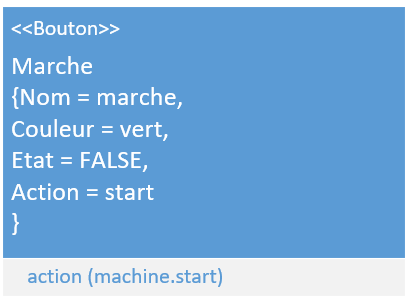
\includegraphics[width=7cm]{10_img/chap4/start.PNG}
    \caption{Une classe pour \texttt{Marche}, spécifiée à l'aide du stéréotype \texttt{Bouton} et des valeurs \'etiquet\'ees.}
    \label{fig.uml_marche}
    \end{center}
\end{figure}

\gt{Dans la figure 4.5: les noms des stéréotypes et classes débutent par une majuscule, mais pas les attributs, qui doivent débuter par une minuscule: nom, couleur, etat, action.}

\gt{Voir mon courriel: en UML 2.0, il semble que les tagged values
doivent être mises dans une sous-boite, avec le nom du stéréotype.}

\gt{Ci-haut: les explications portent sur l'ancien exemple, pas le
nouveau avec le Bouton, donc à réécrire.}

\gt{Je crois, comme indiqu\'e plus haut, qu'une utilisation de Bouton serait pr\'ef\'erable.}

%\newpage

\section{Les contraintes}
Les contraintes sont des propriétés spécifiques, qui permettent de sp\'ecifier des conditions additionnelles sur un modèle.
Ces conditions peuvent être appliquées à une ou plusieurs classes, à un ou plusieurs attributs, à une ou plusieurs relations entre classes.
Une contrainte est représent\'ee, dans un modèle, sous la forme d'une note indiquant une phrase qui exprimant la contrainte entre crochets ou encore, de fa\c{c}on plus formelle, sous la forme d'une contrainte OCL~\cite{OCL}.

\subsection*{Exemple}
%
\eh{J'ai placé un [H] sur cette figure car elle passe dans la subsection précédente. cela pose un probleme de compréhension}
\begin{figure}[H]
    \begin{center}
    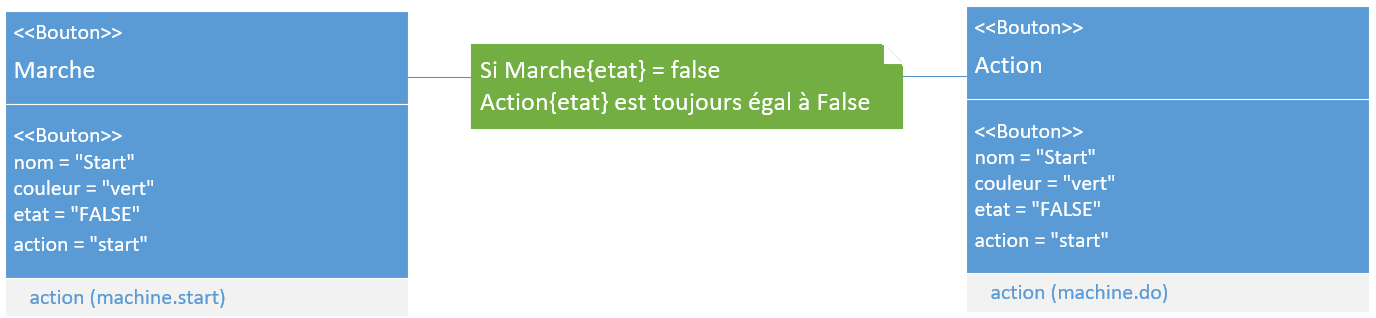
\includegraphics[width=\linewidth]{10_img/chap4/constraint.PNG}
    \caption{Des contraintes sp\'ecifiant des conditions sur des \'el\'ements d'un modèle.}
    \label{fig.uml_con}
    \end{center}
\end{figure}

\gt{Dans la figure: Etat => etat (attribut, minuscule), Nom => nom,
etc. Et j'écrirais plutôt <<Si Marche(etat) = false Alors Action(etat)
= false>>}

Nous trouvons l'exemple d'une contrainte dans la Figure~\ref{fig.uml_con}, entre les boutons \texttt{Marche} et \texttt{Action}.
Cette contrainte énonce que si l'état du bouton \texttt{Marche} est \texttt{false}, alors l'état du bouton \texttt{Action} sera lui aussi \texttt{false},
ce qui signifie que l'action de la machine ne peut pas être effectuée si la machine est à l'arrêt.
On pourra alors sp\'ecifier, dans un diagramme UML, la contrainte présent\'ee dans la figure~\ref{fig.uml_con}.

%\newpage

\section{Les ic\^ones}
Lorsque la taille d'un modèle devient importante, il peut devenir difficile de s'y retrouver parmi les nombreux st\'er\'eotypes.
Dans ce cas, l'association d'ic\^ones aux st\'er\'eotypes peut être une solution int\'eressante à mettre en place dans le cas d'un profil dans un domaine d'activité spécifique.
Une représentation graphique simple --- une ic\^one --- peut ainsi être attribuée à un type d'élément spécifique du modèle.

\subsection*{Exemple}
%
\eh{J'ai placé un [H] sur cette figure car elle passe dans la subsection précédente. cela pose un probleme de compréhension}
\begin{figure}[H]
    \begin{center}
    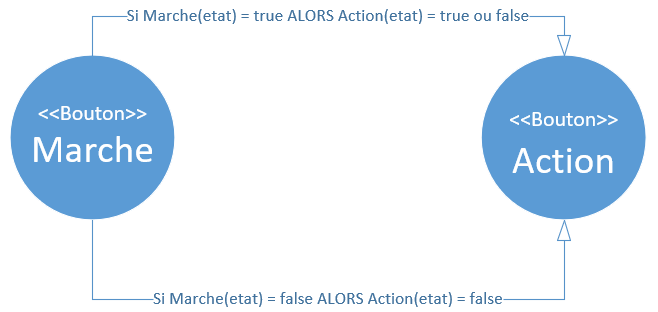
\includegraphics[width=12cm]{10_img/chap4/etat.PNG}
    \caption{Une ic\^one spécifique associ\'ee aux boutons.}
    \label{fig.uml_img}
    \end{center}
\end{figure}

Dans notre exemple, une machine est composée de trois boutons.
On peut alors choisir, par exemple, d'attribuer une ic\^one spécifique aux boutons afin de les différencier des autres éléments, tel qu'illustr\'e dans la figure~\ref{fig.uml_img}.



%\newpage

\section{L'utilisation d'un profil UML pour la conception de jeux vidéos}


UML est un langage de modélisation permettant de représenter divers types de systèmes et permettant de les documenter de manière rigoureuse en apportant les caractéristiques suivantes :

\begin{itemize}
    \item UML est un langage formel et normalisé;
    \item UML est manipulable avec de nombreux outils déjà approuvés;
    \item UML est un support de communication performant;
    \item UML est un langage qui permet le contrôle des versions et la conservation de l'information de manière efficace.
\end{itemize}

\gt{Ci-haut: Pas certain que j'aime la comparaison avec les mind maps.
Dans mon esprit, un mind map a un r\^ole tout \`a fait diff\'erent ---
plus exploratoire, parce que plus libre, avec moins de
contraintes. Donc, je crois que tes items pourraient rester, mais sans
insister sp\'ecifiquement que c'est par rapport aux mind maps.}



Cependant, UML est un langage de modélisation tellement étendu qu'il permet de <<tout faire>> --- ou presque ---, ce qui rend le langage difficile à appréhender.
De plus, UML est prévu à l'origine pour représenter des systèmes logiciels quelconques, donc avec un vocabulaire générique.


Dans les chapitres précédents, nous avons établi une liste de points importants concernant la conception de jeux vidéos.
Nous pensons qu'un profil UML serait un outil int\'eressant pour répondre aux besoins de modélisation d'un GDD.
La mise en place d'un profil UML aurait plusieurs avantages :
\begin{itemize}
    \item En utilisant un profil, il est possible de simplifier la compréhension des différents éléments UML utilisés pour exprimer un concept, ce qui permet de réduire la quantité de connaissances à acquérir pour se servir d'UML dans le cadre de la rédaction d'un GDD.

    \item Les stéréotypes permettent d'intégrer des notions spécifiques au \emph{game design}.

    \item Les valeurs \'etiquet\'ees permettent d'ajouter des propriétés spécifiques aux nouveaux éléments introduits par les st\'er\'eotypes.

    \item Des contraintes peuvent être sp\'ecifi\'ees dans un profil afin d'éviter des erreurs.

    \item Des ic\^ones peuvent être associ\'ees aux éléments du modèle pour faciliter sa compréhension.

    \item Les outils supportant UML sont nombreux et efficaces. Ils sont déjà présents sur le marché et répondent aux besoins de la modélisation UML.
\end{itemize}


\gt{Ci-haut: 2e item: je ne comprends l'histoire de <<port\'ee>> des objets!?}

Grâce aux ajustements et extensions permis par les profils, UML semble être un langage int\'eressant pour permettre la représentation graphique d'un GDD.
C'est pourquoi, dans le prochain chapitre, nous proposons un profil UML permettant la description des éléments d'un GDD.

\chapter{Un profile UML pour aider à la rédaction d'un GDD}

\textcolor{red}{Trouver une manière d'introduire le chapitre}


\section{}

\textcolor{red}{Trouver une manière d'introduire le chapitre}
Ne modifient pas le metamodele
Un profile étend le metamodel existant via des stereotypes, des tagged values et des contraintes.
Pas possible de modifier les contraintes déjà existantes mais permet l'adaptation et la custromisation d'éléments existants du metamodel
Les customisations sont définies dans un profile qui est ensuite appliqué à un package.
Il est possible d'appliquer les profiles dynamiquement aux modeles et ils peuvent également être combinés pour appliquer plusieurs profiles simultanés au même modèle.
%%%%%%%%%%%%%%%%%%%%%%%%%%%%%%%%%%%%%%%%%%%%%%%%%%%%%%%%%%%%%%%%%%%%%%%%%%
\begin{comment}
\chapter{Un langage de modélisation pour l'établissement d'un Game Design Document}

\section{Le concept}
\subsection{Définition}
\subsubsection{Quoi ?}
Un langage permettant de modéliser et stocker des idées lors des phases de Breakthrough et de Conception d'un projet de jeu vidéo. La modélisation peut être graphique et/ou textuelle avec application des modifications en parallèle. \\
Les informations peuvent contenir tout le nécessaire pour exprimer les idées (textes, informations numériques, chemins de fichiers...). Les champs peuvent être personalisables pour permettre de la souplesse aux utilisateurs.

\subsubsection{Pour quoi faire ?}
\paragraph{Des outils de modélisation existent pour tous les domaines reliés au développement de logiciels. Ils sont souvent spécifiques à un corps de métier afin de pouvoir proposer un maximum de fonctionnalités spécifiques sans devenir trop compliqué et en utilisant un vocabulaire précis qui correspond au corps de métier concerné.}

\paragraph{Il y a peu ou pas de langages de modélisation plus généraux pour des domaines multi-métiers. Le but est de pouvoir modéliser la réflexion créative en fournissant un élément visuel permettant de mind-mapper les idées, les stocker et les réutiliser. \\
Il faut que la modélisation soit assez souple pour pouvoir répondre aux besoins de chacun des corps de métier d'où le fait que les éléments et attributs peuvent avoir des identifiants spécifiques définis librement par l'utilisateur.}

\subsubsection{Pour quelles raisons ?}
\paragraph{Les supports de réflexion actuellement utilisés : cahier des charges, réunions, notes écrites, mails, minds-maps... L'organisation de ces différents supports dans un ensemble cohérent est tr;s compliqué. Dans un cahier des charges il est compliqué de classer les idées à la volée. Un mind-map nécessite une numérisation ou une retranscription sur un outil de mind-mapping qui sont toutes les deux des techniques non péreines et risquées dans la conservation des données. Des notes écrites peuvent se perdre et n'ont pas de durabilité sur le long terme. Des mails sont péreins mais il est difficile de les organiser pour le stockage de l'information.}
\paragraph{Un langage de modélisation graphique et textuel permettrait de mind-mapper les idées à la volée sous forme de cubes contenant les données nécessaires. La hiérarchisation des éléments permettrait de gérer des héritages et des relations ainsi que d'éviter la répétition trop abondante des mêmes informations. Les faces des cubes permettrait d'isoler les informations nécessaires à chacun des corps de métier.}
\end{comment}
\chapter{Exemple d'application du langage}
\section{PlayerUnknown's Battlegrounds (PUBG)\cite{wikipubg}}

PUBG est un jeu vidéo sortit en 2017 avec des millions de joueurs à travers le globe. Développé par PUBG Corporation (filiale de Bluehole, Inc. ou plus récemment de Krafton Game Union) en 2017 c'est un des premiers jeu standalone permettant à ses joueurs de participer à un "last man standing game" suivi de prêt par Fortnite (Epic Games). Ces deux jeux ont été les deux premiers standalone à populariser le Battle Royale et à le mettre à la portée de tous sans devoir développer ou installer des mods dans des jeux existants.

\subsection{L'origine du Battle Royale}
Le Battle Royale trouve ses racines dans le roman Battle Royale et son adaptation cinématographique. Un programme militaire de simulation de combat prend place da ns une République socialiste d'Extrême Orient complètement coupée du monde extérieur sans aucun droits civiques et extrêmement stable politiquement. Le programme consiste à un tirage au sort annuel de 50 classes de troisième qui sont déplacées chacune vers une zone de combat. Au début de l'expérience tous les élèves sont réunis afin d'obtenir un briefing rapide de l'événement et se voient attribuer un sac contenant un objet (allant d'une arme à feu, à une arme blanche, à une fourchette ou une corde de luth). Ils sont ensuite livrés à eux-mêmes dans une zone donnée en ayant pour seule information : aucune règle n'est imposée et un seul survivant par groupe pourra être gagnant de l'expérience les autres devront être exterminés par n'importe quel moyen à disposition. Le champion obtient le droit de vivre aux frais de l'État pour le reste de ses jours et la reconnaissance comme Héros du pays.

\subsection{La naissance de la popularité du Battle Royale}
L'intérêt pour le principe du Battle Royale n'explose que plus tard avec le succès de la saga Hunger Games mettant en place l'histoire de Katniss Everdeen, une jeune adulte qui participe de son plein gré aux Hunger Games. Dans un État totalitaire séparé en castes regroupées dans des districts, deux enfants et/ou adolescents sont choisis au hasard dans chaque district afin de devenir les Tribus. Ils sont alors réunis à la capitale et lâchés dans une arène afin de participer à une télé-réalité de match à mort diffusée partout dans le pays.
Son succès a amené les développeurs du jeu Arma II à créer un mode de jeu basé sur les mêmes règles. Ce mode sera alors appelé DayZ et deviendra par la suite un jeu standalone. Un mode voit également le jour : Battle Royale. Développé par Brendan Greene pour Arma II et ensuite Arma III, ce mode gagne suffisament en popularité pour que celui-ci donne naissance au projet de jeu PlayerUnknown's Battlegrounds (PlayerUnknown étant le pseudonyme en ligne utilisé par Brendan Greene).

\subsection{Les règles de PUBG}
Un avion parcours une ligne droite sur une carte, les 100 joueurs de la partie doivent sauter de cet avion afin d'être parachutés à l'endroit de leur choix à condition qu'il soit à portée. Une fois arrivés au sol, les joueurs partent à la recherche d'armes et d'équipement dans des bâtiments et doivent s'entretuer jusqu'à ce qu'un seul joueur ne soit vivant et gagne ainsi la partie (il est également possible de jouer en duo ou en squad de 4 joueurs ou la dernière équipe debout devient gagnante). Afin de limiter la durée d'une partie, une zone circulaire est définie sur la carte une fois que tous les joueurs ont atterri et celle-ci se réduit par étapes au cours de la partie. Les joueurs en dehors de la zone subissent une certaine quantité de dégâts toutes les secondes s'ils restent en dehors du cercle et ces dégâts augmentent au fur et à mesure que le cercle se resserre.

\subsection{Les Battle Royale dans le monde du jeu vidéo}
Ces dernières années une quantité astronomique de Battle Royale voit le jour dans le jeu vidéo. De Fortnite (Epic Games) à PUBG, en passant par Apex Legends (Respawn Entertainement), Ring of Elysium (Tencent Games) pour ne citer que les plus importants. Des dizaines de jeux voient le jour ou se réinventent afin de coller à la mode des Battle Royale. Les plus grandes licences de FPS (First Personal Shooters) s'alignent également à cette mode, c'est ainsi que voient le jours les modes de jeu Z1BR (H1Z1), Firestorm (Battlefield V), Blackout (Call of Duty Black Ops IV). Mais cette offre répond à une demande phénoménale du public pour ce mode de jeu qui s'impose dans le marché à la même place que le type de jeu MOBA (Multiplayer Online Battle Arena) qui était grand favoris du public depuis une dizaine d'années à travers les jeux League Of Legends ou Dota 2. Avec le temps les Battle Royale tentent de se réinventer et de trouver de nouveaux publics en gardant le principe de Battle Royale mais en apportant d'autres univers. C'est ainsi que naissent Last Tide et son univers aquatique immergé, Fall Guys : Ultimate Knockout et son univers colorés où de petits personnages à la physique étrange se battent pour une couronne, Cuisine Royale, qui était à l'origine une blague de développeurs mais qui a rencontré un succès, dans lequel les personnages se battent à l'aide d'ustensiles de cuisine.

\section{Représentation d'une partie des mécaniques de PUBG}
\subsection{Les données}
Données difficiles à obtenir de façon fiable.
Informatiosn extraites de https://pubg.gamepedia.com/
Wikipedia régulièrement mis a jours
Extraction des informations via les fichiers de jeu minés


\subsection{Le profile}
Arbre des stereotypes découpé avec explications
\begin{figure}[H]
    \centering
    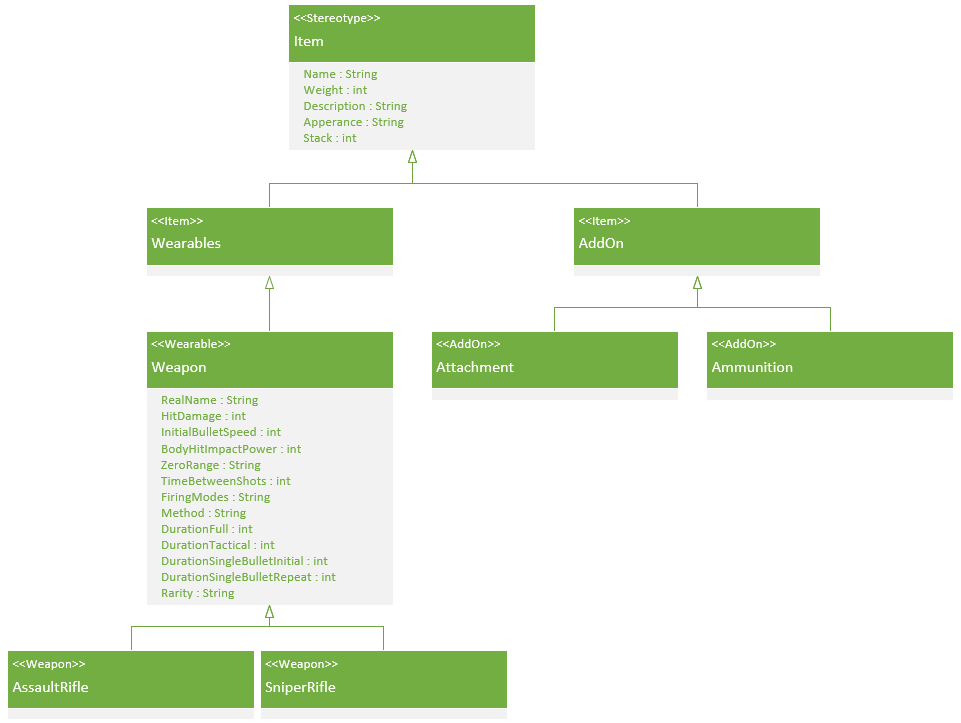
\includegraphics[width=14cm]{10_img/chap6/root(stereotypes).PNG} 
    \caption{Racine des stereotypes concernés par l'exemple}
\end{figure}
Focus sur la section concernée par la partie decrite plus bas (attachments)



\subsection{La modélisation}

\begin{figure}[H]
    \centering
    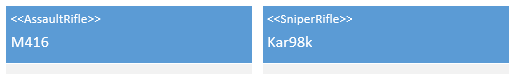
\includegraphics[width=10cm]{10_img/chap6/weapons.PNG} 
    \caption{Classes des "Weapon" concernées par l'exemple}
\end{figure}

\begin{figure}[H]
    \centering
    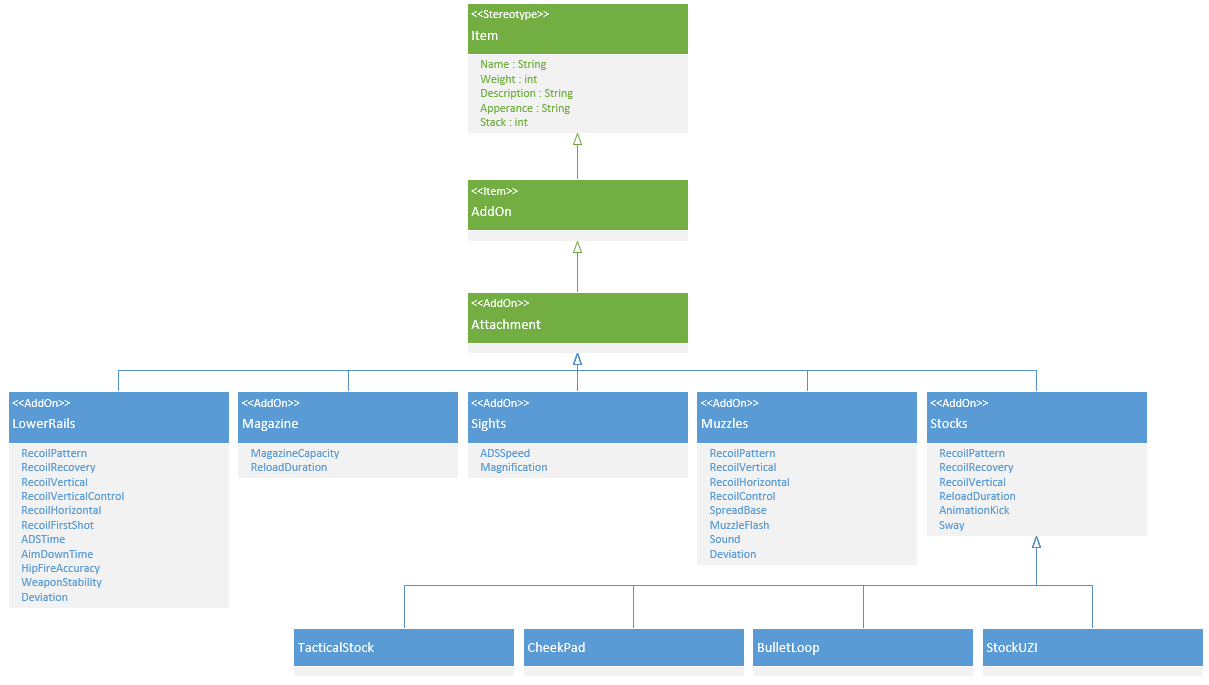
\includegraphics[width=14cm]{10_img/chap6/attachments_stocks.PNG} 
    \caption{Arbre des "Attachment" concernés par l'exemple}
\end{figure}

\begin{figure}[H]
    \centering
    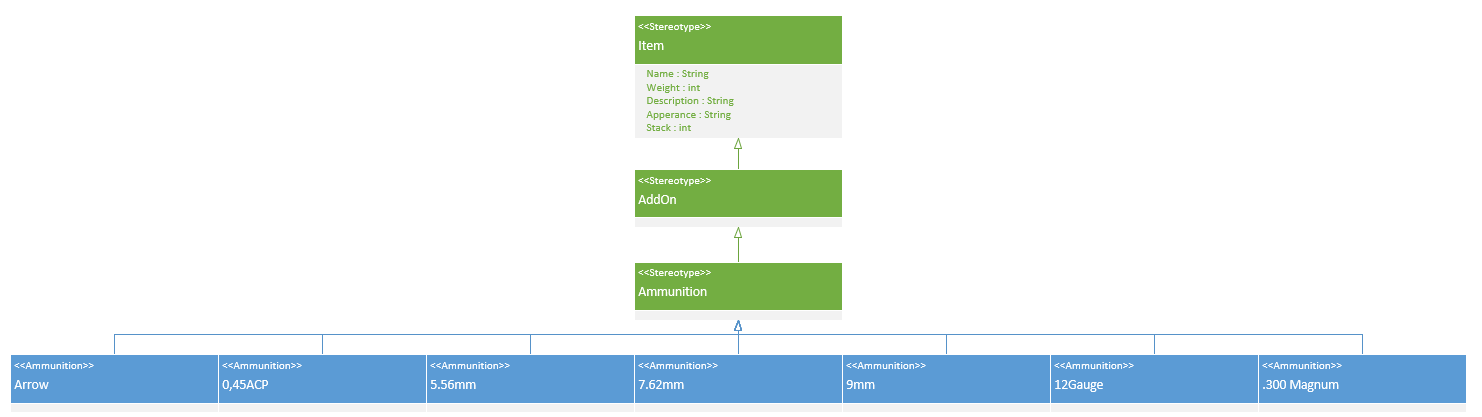
\includegraphics[width=10cm]{10_img/chap6/ammunitions.PNG} 
    \caption{Arbre des "Ammunition" concernés par l'exemple}
\end{figure}


Afin de pouvoir visualiser les interactions entre les éléments il est nécessaire de nommer les associations entre les classes. Afin de mettre en place ces nommages d'associations un groupe de stéréotypes a étét mis en place.


\begin{figure}[H]
    \centering
    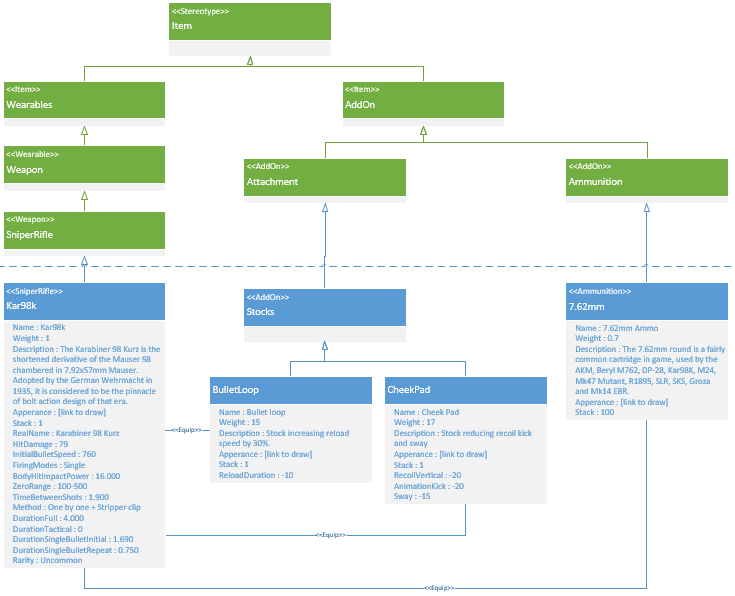
\includegraphics[width=14cm]{10_img/chap6/Kar98k_stock_ammunition_links.PNG} 
    \caption{Arbre du Kar98k, avec ses Stocks et ses Ammunitions concernés par l'exemple}
\end{figure}


\begin{figure}[H]
    \centering
    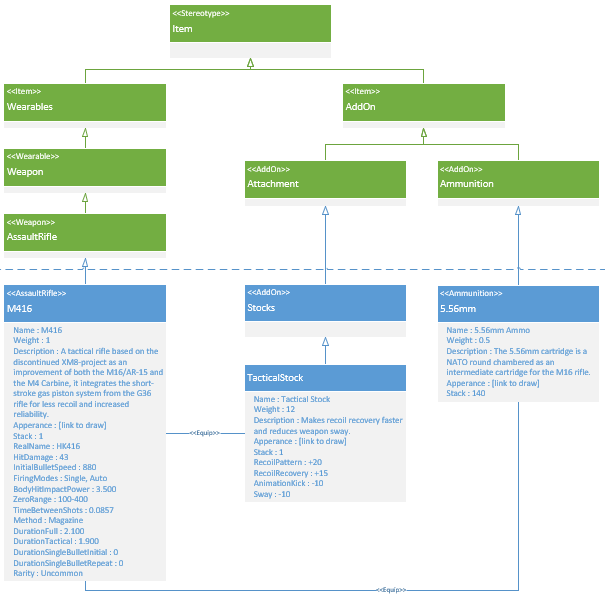
\includegraphics[width=14cm]{10_img/chap6/M416_stock_ammunition_links.PNG} 
    \caption{Arbre du M416, avec ses Stocks et ses Ammunitions concernés par l'exemple}
\end{figure}


\begin{figure}[H]
    \centering
    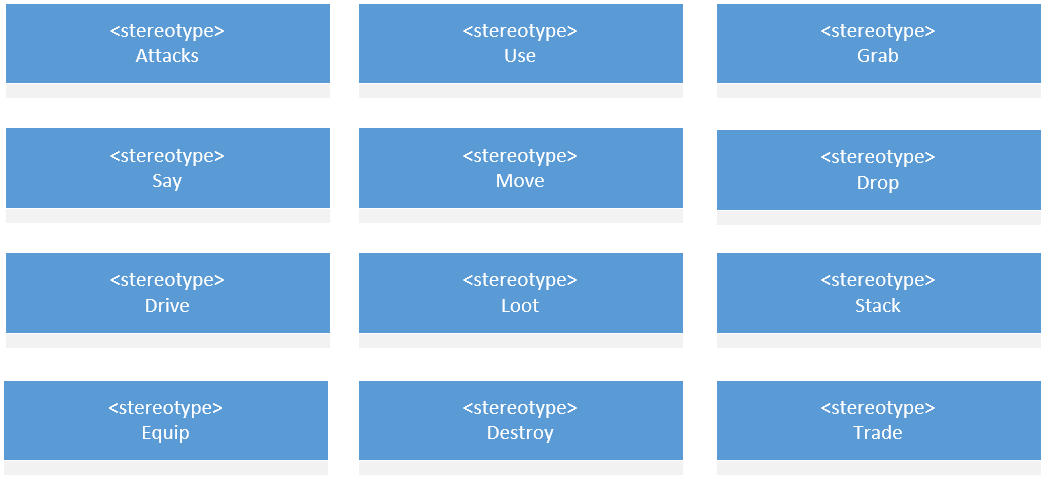
\includegraphics[width=10cm]{10_img/chap6/interacts.PNG} 
    \caption{Arbre des "Interactions" concernées par l'exemple}
\end{figure}

\subsection{Synthèse sous forme de GDD}
Rédaction du GDD avec les informations de la modélisation

\section{Evolutions possibles}
\subsection{Outil de manipulation visuelle du profile UML}
\subsection{Transformation du modèle en GDD}
\subsection{Accélérateur de description des mécaniques}







%%%%%%%%%%%%%%%%%%%%%%%%%%%%%%%%%%%%%%%%%%%%%%%%%%%%%%%%%%%%%%%%%%%%%%%%%%
\begin{comment}
\section{Dans le cadre de Anno1800}
\subsection{Exemple des Mécaniques de Gameplay concernant la Maison d'ouvriers}

\begin{figure}[h!]
    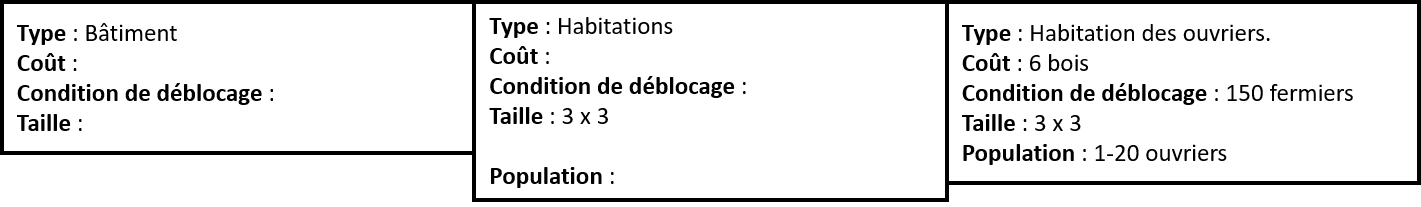
\includegraphics[width=15cm]{10_img/bati_maison_ouvrier.png} 
    \caption{Mécanique de gameplay : Maison d'ouvriers}
\end{figure}

\begin{figure}
    \begin{subfigure}[b]{0.4\textwidth}
        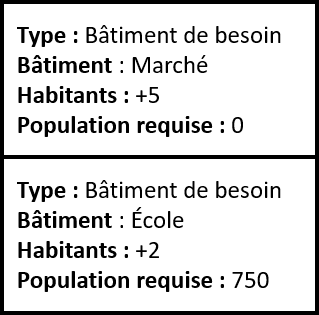
\includegraphics[width=4cm]{10_img/bati_maison_ouvrier_batbesoin.png} 
        \caption{Maison d'ouvriers - Bâtiments de besoins}
    \end{subfigure}
        \hfill
    \begin{subfigure}[b]{0.5\textwidth}
        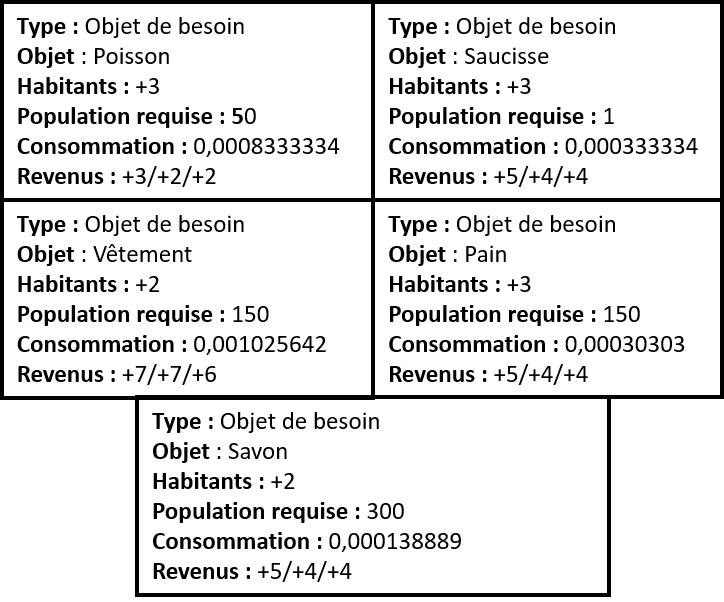
\includegraphics[width=7cm]{10_img/bati_maison_ouvrier_objbesoin.png} 
        \caption{Maison d'ouvriers - Ressources de besoins}
    \end{subfigure}
        \hfill
    \begin{subfigure}[b]{0.4\textwidth}
        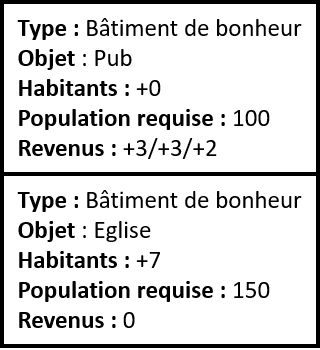
\includegraphics[width=4cm]{10_img/bati_maison_ouvrier_bathonneur.png} 
        \caption{Maison d'ouvriers - Bâtiments de bonheur}
    \end{subfigure}
        \hfill
    \begin{subfigure}[b]{0.4\textwidth}
        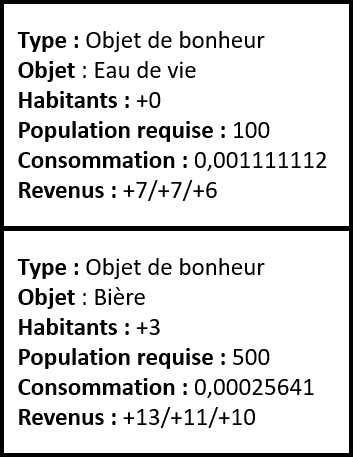
\includegraphics[width=4cm]{10_img/bati_maison_ouvrier_objbonheur.png} 
        \caption{Maison d'ouvriers - Ressources de bonheur}
    \end{subfigure}
    \caption{Mécanique de gameplay : Détails des ressources et bâtiments de besoin et de bonheur}\label{fig:animals}
\end{figure}

\end{comment}


\begin{conclusion}

%le but => Faciliter la modélisation des mecha dans le proc de pre conception d'un jv
Un projet de développement informatique est une tâche de longue haleine rythmée par de nombreux changements,
et
la description des concepts et la conception sont essentielles au bon déroulement du projet ainsi qu'à sa réussite.
%
Ceci encore plus marqué dans le domaine des jeux vidéos car
le développement d'un jeu implique non seulement des développeurs mais également de nombreux autres corps de métier~: artistes (planches pour illustrer les éléments graphiques),  musiciens (bande originale du jeu), modeleurs et animateurs 3D (éléments graphiques), scénaristes (cadre et histoire du jeu), etc.
Réussir à apporter les informations nécessaires à tous ces corps de métier est un défi que le \emph{game designer} affronte au quotidien.

Un document de \emph{game design} est un pilier d'un projet de développement d'un jeu.
Sa rédaction est complexe, chronophage et nécessite une rigueur exemplaire des \emph{game designers}.
Cependant, aucun gabarit préconçu n'existe pour répondre à tous leurs besoins.
Chaque projet est différent, chaque jeu possède des spécificités, chaque équipe de développement est différente et cela empêche l'établissement d'un modèle générique de \emph{Game Design Document}.

Dans la littérature, nous avons identifié plusieurs listes de bonnes pratiques de design, chacune essayant de généraliser ses conseils pour tous les genres de jeu.
C'est le cas du \emph{framework MDA}, qui propose un découpage d'un jeu afin de structurer les différents éléments dans trois catégories et lier ces éléments pour qu'ils fonctionnent ensemble.

Définir tous les éléments d'un système et décrire leurs interactions est une approche déjà présente dans le développement logiciel classique.
C'est ce que l'on retrouve notamment à travers la modélisation UML.
Cependant, UML est un langage générique, conçu pour le développement informatique et il est donc compliqué pour les autres corps de métier d'acquérir les connaissances nécessaires à sa compréhension.
Il est cependant possible de créer des profils UML afin d'adapter les modèles UML et les étendre pour intégrer un vocabulaire spécifique à un domaine d'activité particulier.

Une fois le vocabulaire adapté à la conception de jeux vidéos, UML a la capacité d'apporter plusieurs avantages.
UML est un langage formel, permettant la description de systèmes et de processus, efficace, extensible et largement documenté.
Les outils qui l'accompagnent sont fiables et respectent une rigueur qui permet la réutilisation des modèles et en respectant le contenu des données.
Sa formalisation permet également d'assurer la pérennité des modèles dans le temps et leur cohérence, peu importe le nombre de modifications et la durée de leur utilisation.

\gt{Il faut mettre un tilde <<\~{}>> devant $\backslash$ref et
$\backslash$cite, mais pas $\backslash$emph!}


\gt{Ci-bas: encore <<pré>>-conception, qui n'apparaît pas dans les étapes du chapitre I!}

C'est ce que nous recherchions dans notre problématique : apporter une description fiable, modifiable, compréhensible et précise dans la conception d'un jeu vidéo et la rédaction de son \emph{Game Design Document}.
%
Et c'est dans cette optique que nous avons conçu \emph{Game Genesis}, un profil UML intégrant un vocabulaire adapté à la conception de jeux vidéos dans des modèles UML.
%
Pour ce faire, 
nous avons étudié différents \emph{Game Design Documents} afin de définir des caractéristiques communes à ces documents.
Nous nous sommes concentrés sur la modélisation des éléments de \emph{Mechanics} présents dans ces documents afin d'établir une liste des éléments qui se retrouvent dans de nombreux genres et donc de nombreux projets de développement de jeux vidéos.
Une fois cette liste établie, nous avons proposé une liste de stéréotypes correspondant à ces éléments, 
liste dont les éléments ont été organisés selon une structure hiérarchique afin de les classifier dans des catégories conceptuelles appropriées.
Afin de représenter, cette hiérarchie nous avons utilisé le mécanisme d'héritage d'UML.
Ceci nous a permis de définir des caractéristiques dans les catégories et les éléments qui leur sont associés héritent des attributs.

Afin de décrire les interactions entre les éléments de \emph{Mechanics}, nous avons utilisé des associations.
Les stéréotypes de \emph{Game Genesis} comprennent donc une catégorie \texttt{Interaction} dont les éléments s'appliquent sur les associations UML.
Ces stéréotypes décrivent des interactions entre éléments et peuvent porter des attributs et méthodes.

Finalement, nous avons exploré l'utilisation du profil \emph{Game Genesis} dans un exemple à travers le jeu \emph{PlayerUnknown's BattleGrounds} (PUBG).
Nous avons modélisé certains des concepts clés d'une partie de ce jeu en utilisant un diagramme de classes sur lequel était appliqué le profil \emph{Game Genesis}.
Donc, plus spécifiquement, avec ce modèle, nous avons décrit une partie des éléments de \emph{Mechanics} du jeu PUBG et certaines de leurs interactions.

\emph{Game Genesis} ne se concentre que sur la description des éléments de \emph{Mechanics} d'un jeu.
Or, ce n'est qu'une partie du design d'un jeu, de la rédaction d'un \emph{Game Design Document} et du \emph{Framework MDA}.
Nous nous sommes concentrés sur ces éléments de façon à limiter l'envergure du travail, car la représentation de tous les éléments du \emph{framework MDA} aurait été trop complexe à réaliser dans le cadre d'un travail de maîtrise.
%
On peut toutefois envisager que d'autres types de diagrammes UML
puissent être utilisés pour le \emph{design} de jeux, notamment
pour la description des éléments de \emph{Dynamics}.

La représentation des éléments et concepts d'un jeu dans un diagramme de classes ouvre de nombreuses possibilités pour la rédaction de \emph{Game Design Documents}.
En effet, il est possible de réutiliser les modèles, et UML étant un langage informatique, il est possible de le manipuler et de générer d'autres documents.
En réutilisant les modèles, il serait possible d'extraire des informations des modèles afin de générer le début d'un \emph{Game Design Document} décrivant les éléments de \emph{Mechanics} du jeu en question.
Il serait également possible de générer un squelette d'application à partir des modèles, un diagramme de classes étant tout indiqué pour cette transformation.
Nous pourrions aussi imaginer un outil de gestion des versions permettant de faire un différentiel entre les différentes versions des modèles.
Il serait alors possible de stocker les justifications d'une modification effectuée et documenter ces modifications pour le futur.
%
Par contre, toutes ces possibilités sont pour l'instant des pistes car \emph{Game Genesis} est aujourd'hui à l'état de preuve de concept.
Ces possibles évolutions demandent que notre profil
\emph{Game Genesis} soit incorporé de façon effective dans un outil
UML existant, ce que nous n'avons pas eu le temps de faire, et qui
serait une piste intéressante pour un travail futur.


\gt{Ci-haut: il faut aussi dire quelques mots sur une autre limitation
--- il vaut mieux le dire explicitement, plutôt que se le faire dire
par un examinateur: ce que tu as fait est une sorte de prototype ou
preuve de concept exploratoire, en ce sens que ce profil n'a pas été
inclus de façon effective dans un vrai outil UML.  C'est aussi une
piste de travail futur à mentionner.}

\gt{Et ci-bas: il ne faut pas trop dire que c'est vraiment un outil,
car beaucoup plus une preuve de concept pour l'instant. Peut-être plus
des <<pistes intéressantes>>?}


Finalement, nous espérons que cette recherche aura permis d'identifier des pistes intéressantes et nouvelles pour concevoir un outil adapté au domaine du développement de jeux vidéos, avec comme objectif d'apporter une représentation graphique des éléments de \emph{Mechanics} --- et possiblement de \emph{Dynamics} --- et  permettant de structurer et de documenter le processus de conception et d'accompagner les \emph{game designers} dans leur tâche.


%la nature et l’envergure du travail
%les sujets traités => Dev jv, gdd, mda, profils
%les problèmes à résoudre => formaliser une représentation des Mecha, faciliter la representation, 
%les objectifs fixés => apporter un outil fiable, langage adapté aux JV, malléable pour tous les gameplay, 
%les méthodes utilisées => profil UML,Établir un profil UML pour représenter les éléments de Mechanics dans le processus de pré-conception d'un JV
%la démarche adoptée => GDD (exemples et bonnes pratiques), MDA (section Mecha), Profil UML
%les résultats les plus saillants => Exemple d'application ok, possibilité de decrire les mecha et leurs relations efficacement
%les limites et les conclusions => Représentation des Mecha (no dyna no aesth)
%les recommandations et les pistes de recherche => utilisation des modeles générés pour : générer un squelette de GDD, générer un squelette de code, stocker les données pour le versionning


\end{conclusion}



% Utilisez l'environnement  conclusion pour rédiger votre conclusion


\chapter*{ANNEXE A}
\addcontentsline{toc}{chapter}{ANNEXE A}  

\section*{Item}
\addcontentsline{toc}{section}{Item}  
\begin{figure}[H]
    \centering
    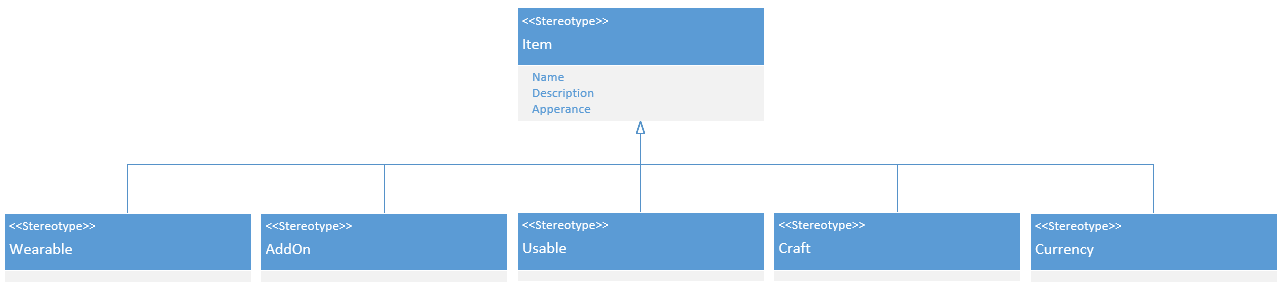
\includegraphics[width=14cm]{10_img/chap5/01_00_item.PNG} 
    \caption{TITRE}
\end{figure}
\begin{figure}[H]
    \centering
    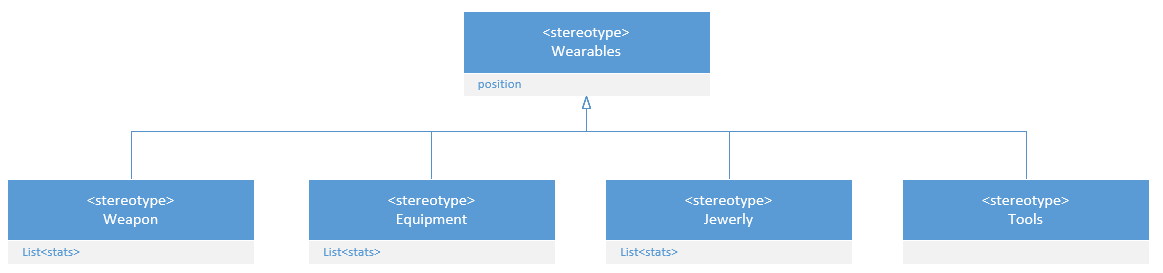
\includegraphics[width=14cm]{10_img/chap5/01_01_wearable.PNG} 
    \caption{TITRE}
\end{figure}
\begin{figure}[H]
    \centering
    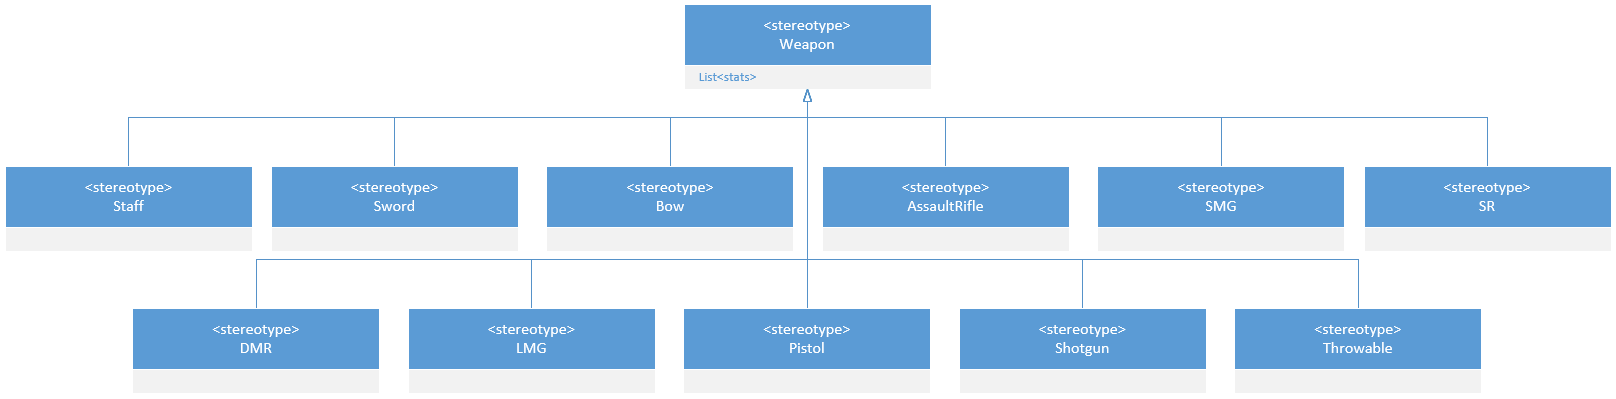
\includegraphics[width=14cm]{10_img/chap5/01_01_01_weapon.PNG} 
    \caption{TITRE}
\end{figure}
\begin{figure}[H]
    \centering
    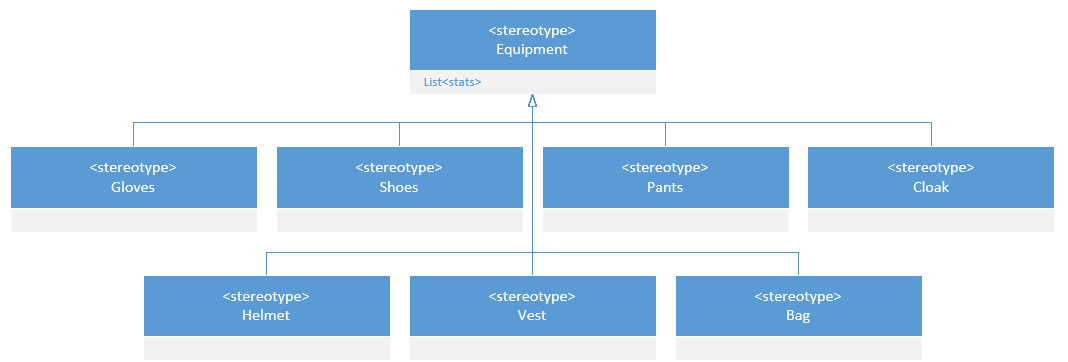
\includegraphics[width=14cm]{10_img/chap5/01_01_02_equipment.PNG} 
    \caption{TITRE}
\end{figure}
\begin{figure}[H]
    \centering
    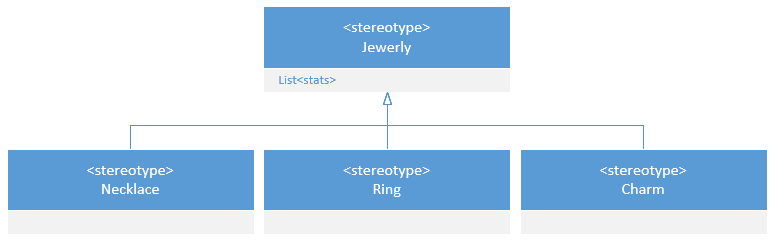
\includegraphics[width=14cm]{10_img/chap5/01_01_03_jewerly.PNG} 
    \caption{TITRE}
\end{figure}
\begin{figure}[H]
    \centering
    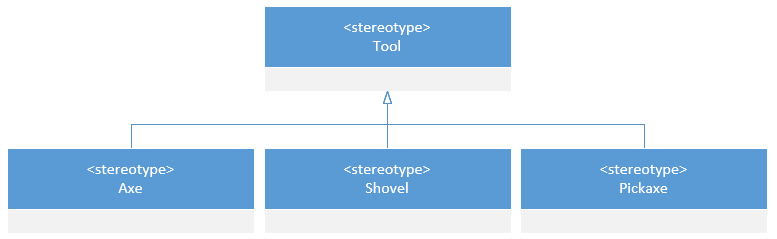
\includegraphics[width=14cm]{10_img/chap5/01_01_04_tool.PNG} 
    \caption{TITRE}
\end{figure}
\begin{figure}[H]
    \centering
    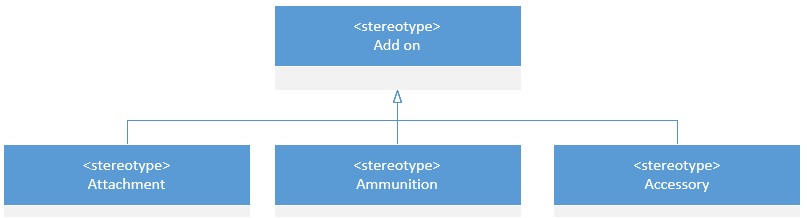
\includegraphics[width=14cm]{10_img/chap5/01_03_addon.PNG} 
    \caption{TITRE}
\end{figure}
\begin{figure}[H]
    \centering
    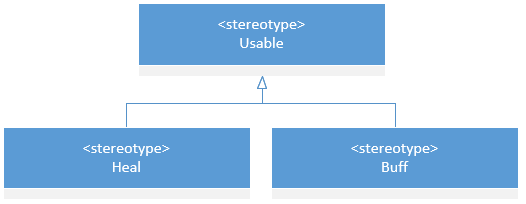
\includegraphics[width=14cm]{10_img/chap5/01_04_usable.PNG} 
    \caption{TITRE}
\end{figure}
\begin{figure}[H]
    \centering
    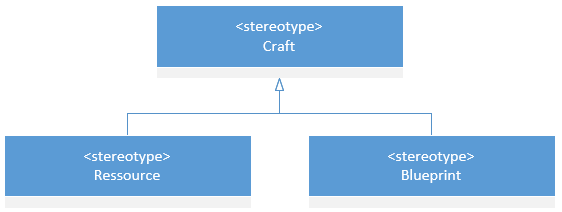
\includegraphics[width=14cm]{10_img/chap5/01_05_craft.PNG} 
    \caption{TITRE}
\end{figure}
\begin{figure}[H]
    \centering
    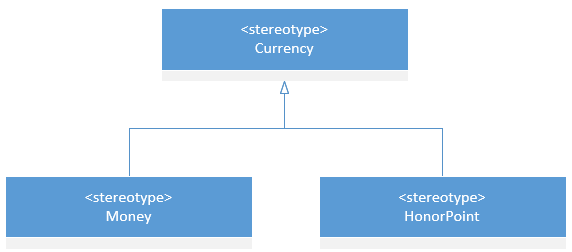
\includegraphics[width=14cm]{10_img/chap5/01_06_currency.PNG} 
    \caption{TITRE}
\end{figure}


\section*{Animate}
\addcontentsline{toc}{section}{Animate}  
\begin{figure}[H]
    \centering
    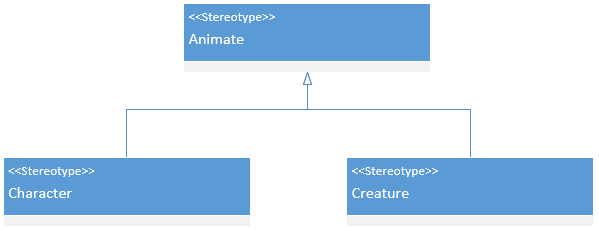
\includegraphics[width=14cm]{10_img/chap5/02_00_animate.PNG} 
    \caption{TITRE}
\end{figure}
\begin{figure}[H]
    \centering
    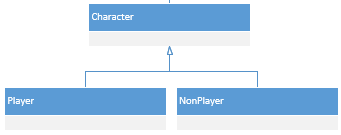
\includegraphics[width=14cm]{10_img/chap5/02_00_01_character.PNG} 
    \caption{TITRE}
\end{figure}
\begin{figure}[H]
    \centering
    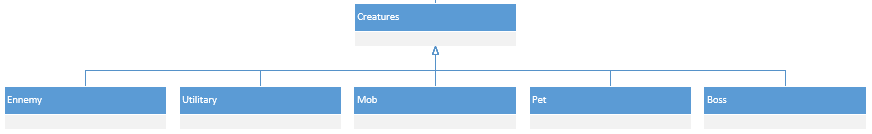
\includegraphics[width=14cm]{10_img/chap5/02_00_02_creature.PNG} 
    \caption{TITRE}
\end{figure}



\section*{Character Sheet}
\addcontentsline{toc}{section}{Character Sheet}  
\begin{figure}[H]
    \centering
    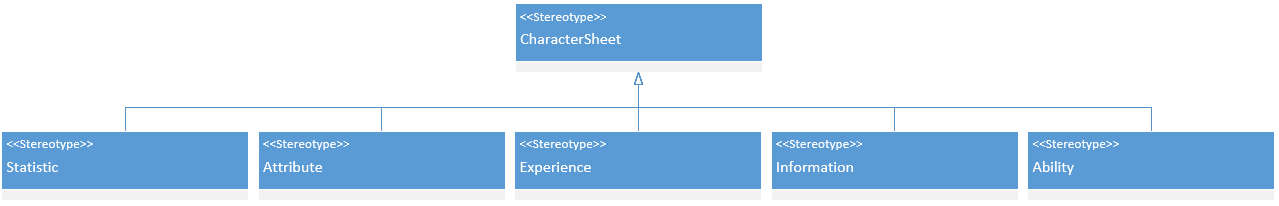
\includegraphics[width=14cm]{10_img/chap5/03_00_charactersheet.PNG} 
    \caption{TITRE}
\end{figure}
\begin{figure}[H]
    \centering
    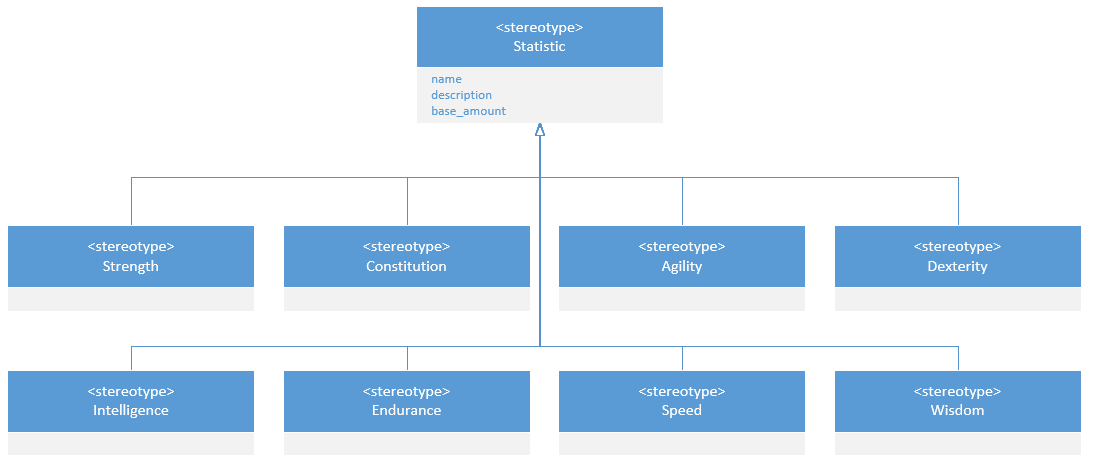
\includegraphics[width=14cm]{10_img/chap5/03_00_01_statistic.PNG} 
    \caption{TITRE}
\end{figure}
\begin{figure}[H]
    \centering
    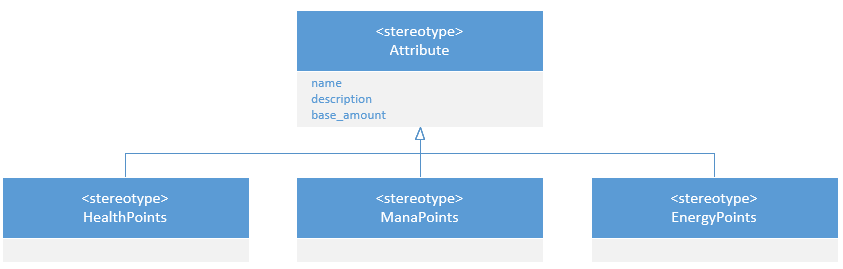
\includegraphics[width=14cm]{10_img/chap5/03_00_02_attribute.PNG} 
    \caption{TITRE}
\end{figure}
\begin{figure}[H]
    \centering
    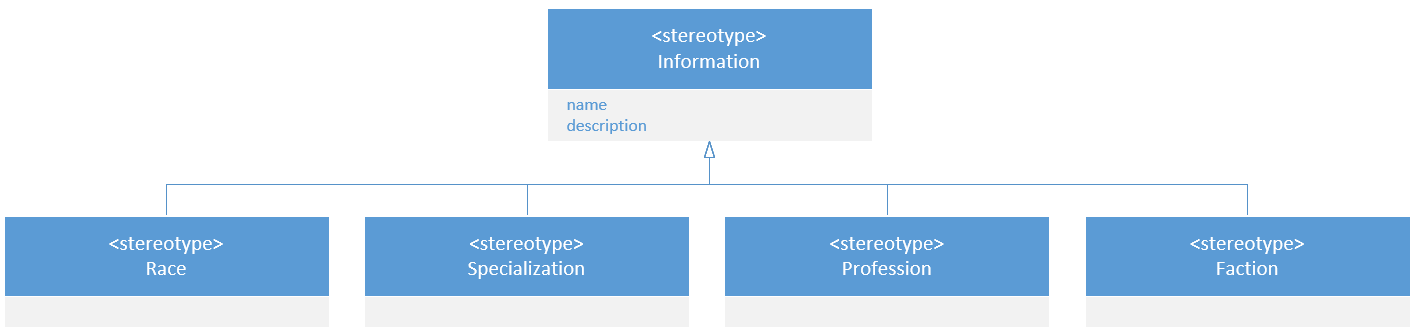
\includegraphics[width=14cm]{10_img/chap5/03_00_03_information.PNG} 
    \caption{TITRE}
\end{figure}


\section*{LORE}
\addcontentsline{toc}{section}{LORE}  
\begin{figure}[H]
    \centering
    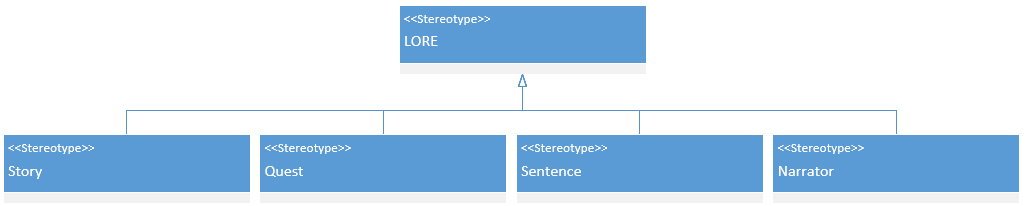
\includegraphics[width=14cm]{10_img/chap5/04_00_lore.PNG} 
    \caption{TITRE}
\end{figure}


\section*{World}
\addcontentsline{toc}{section}{World}  
\begin{figure}[H]
    \centering
    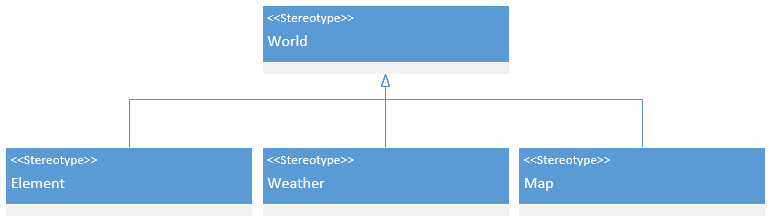
\includegraphics[width=14cm]{10_img/chap5/05_00_world.PNG} 
    \caption{TITRE}
\end{figure}


\section*{Interaction}
\addcontentsline{toc}{section}{Interaction}  
\begin{figure}[H]
    \centering
    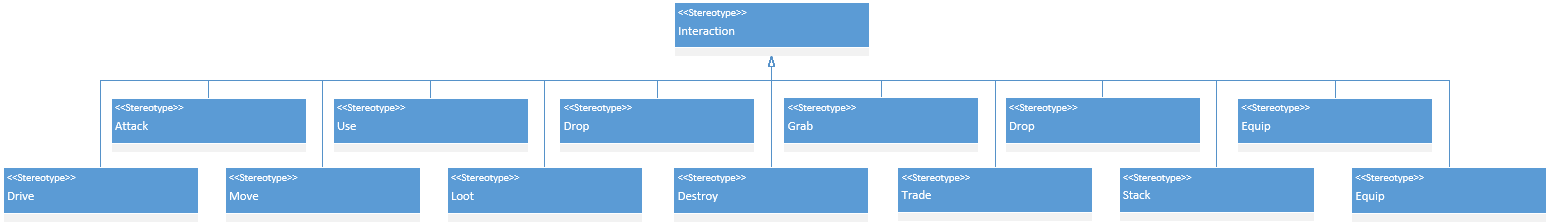
\includegraphics[width=14cm]{10_img/chap5/06_00_interaction.PNG} 
    \caption{TITRE}
\end{figure}

%%%%%%%%%%%%%%%%%%%%
% Page liminaires
%%%%%%%%%%%%%%%%%%%%
\bibliographystyle{apalike-uqam}
\bibliography{03_post/bib}

\end{document}
